This chapter presents and interprets the results of classical simulations of the non-variational quantum walk-based optimisation algorithm (NVQWOA) applied to the unlabelled graph similarity problem. The primary objective is to evaluate the performance of NVQWOA in amplifying the probability of optimal and near-optimal solutions, to examine how its dynamics reflect the structure of the solution space, and to understand how its limited hyperparameter set interacts with different objective functions.

When referring to the hyperparameter optimisation objective functions explained in section \ref{sec:parameters}, we use the acronyms EV for expectation value, OSP for optimal solution probability, and CVaR for conditional value at risk.

\section{Single Graph Analysis}
The first part of the analysis was performed on a randomly chosen graph. The seed 2025 was arbitrarily chosen to create a random graph by the method described in section \ref{sec:problem const}. The NVQWOA was applied to this graph with fixed initial hyperparameters, $\gamma=1.0, t=0.1, \beta=0.4$, in order to see if suboptimal hyperparameters can still produce amplification. The number of iterations was increased to $p=30$.

\begin{figure}[htbp]
\centering
\begin{subfigure}{0.45\textwidth}
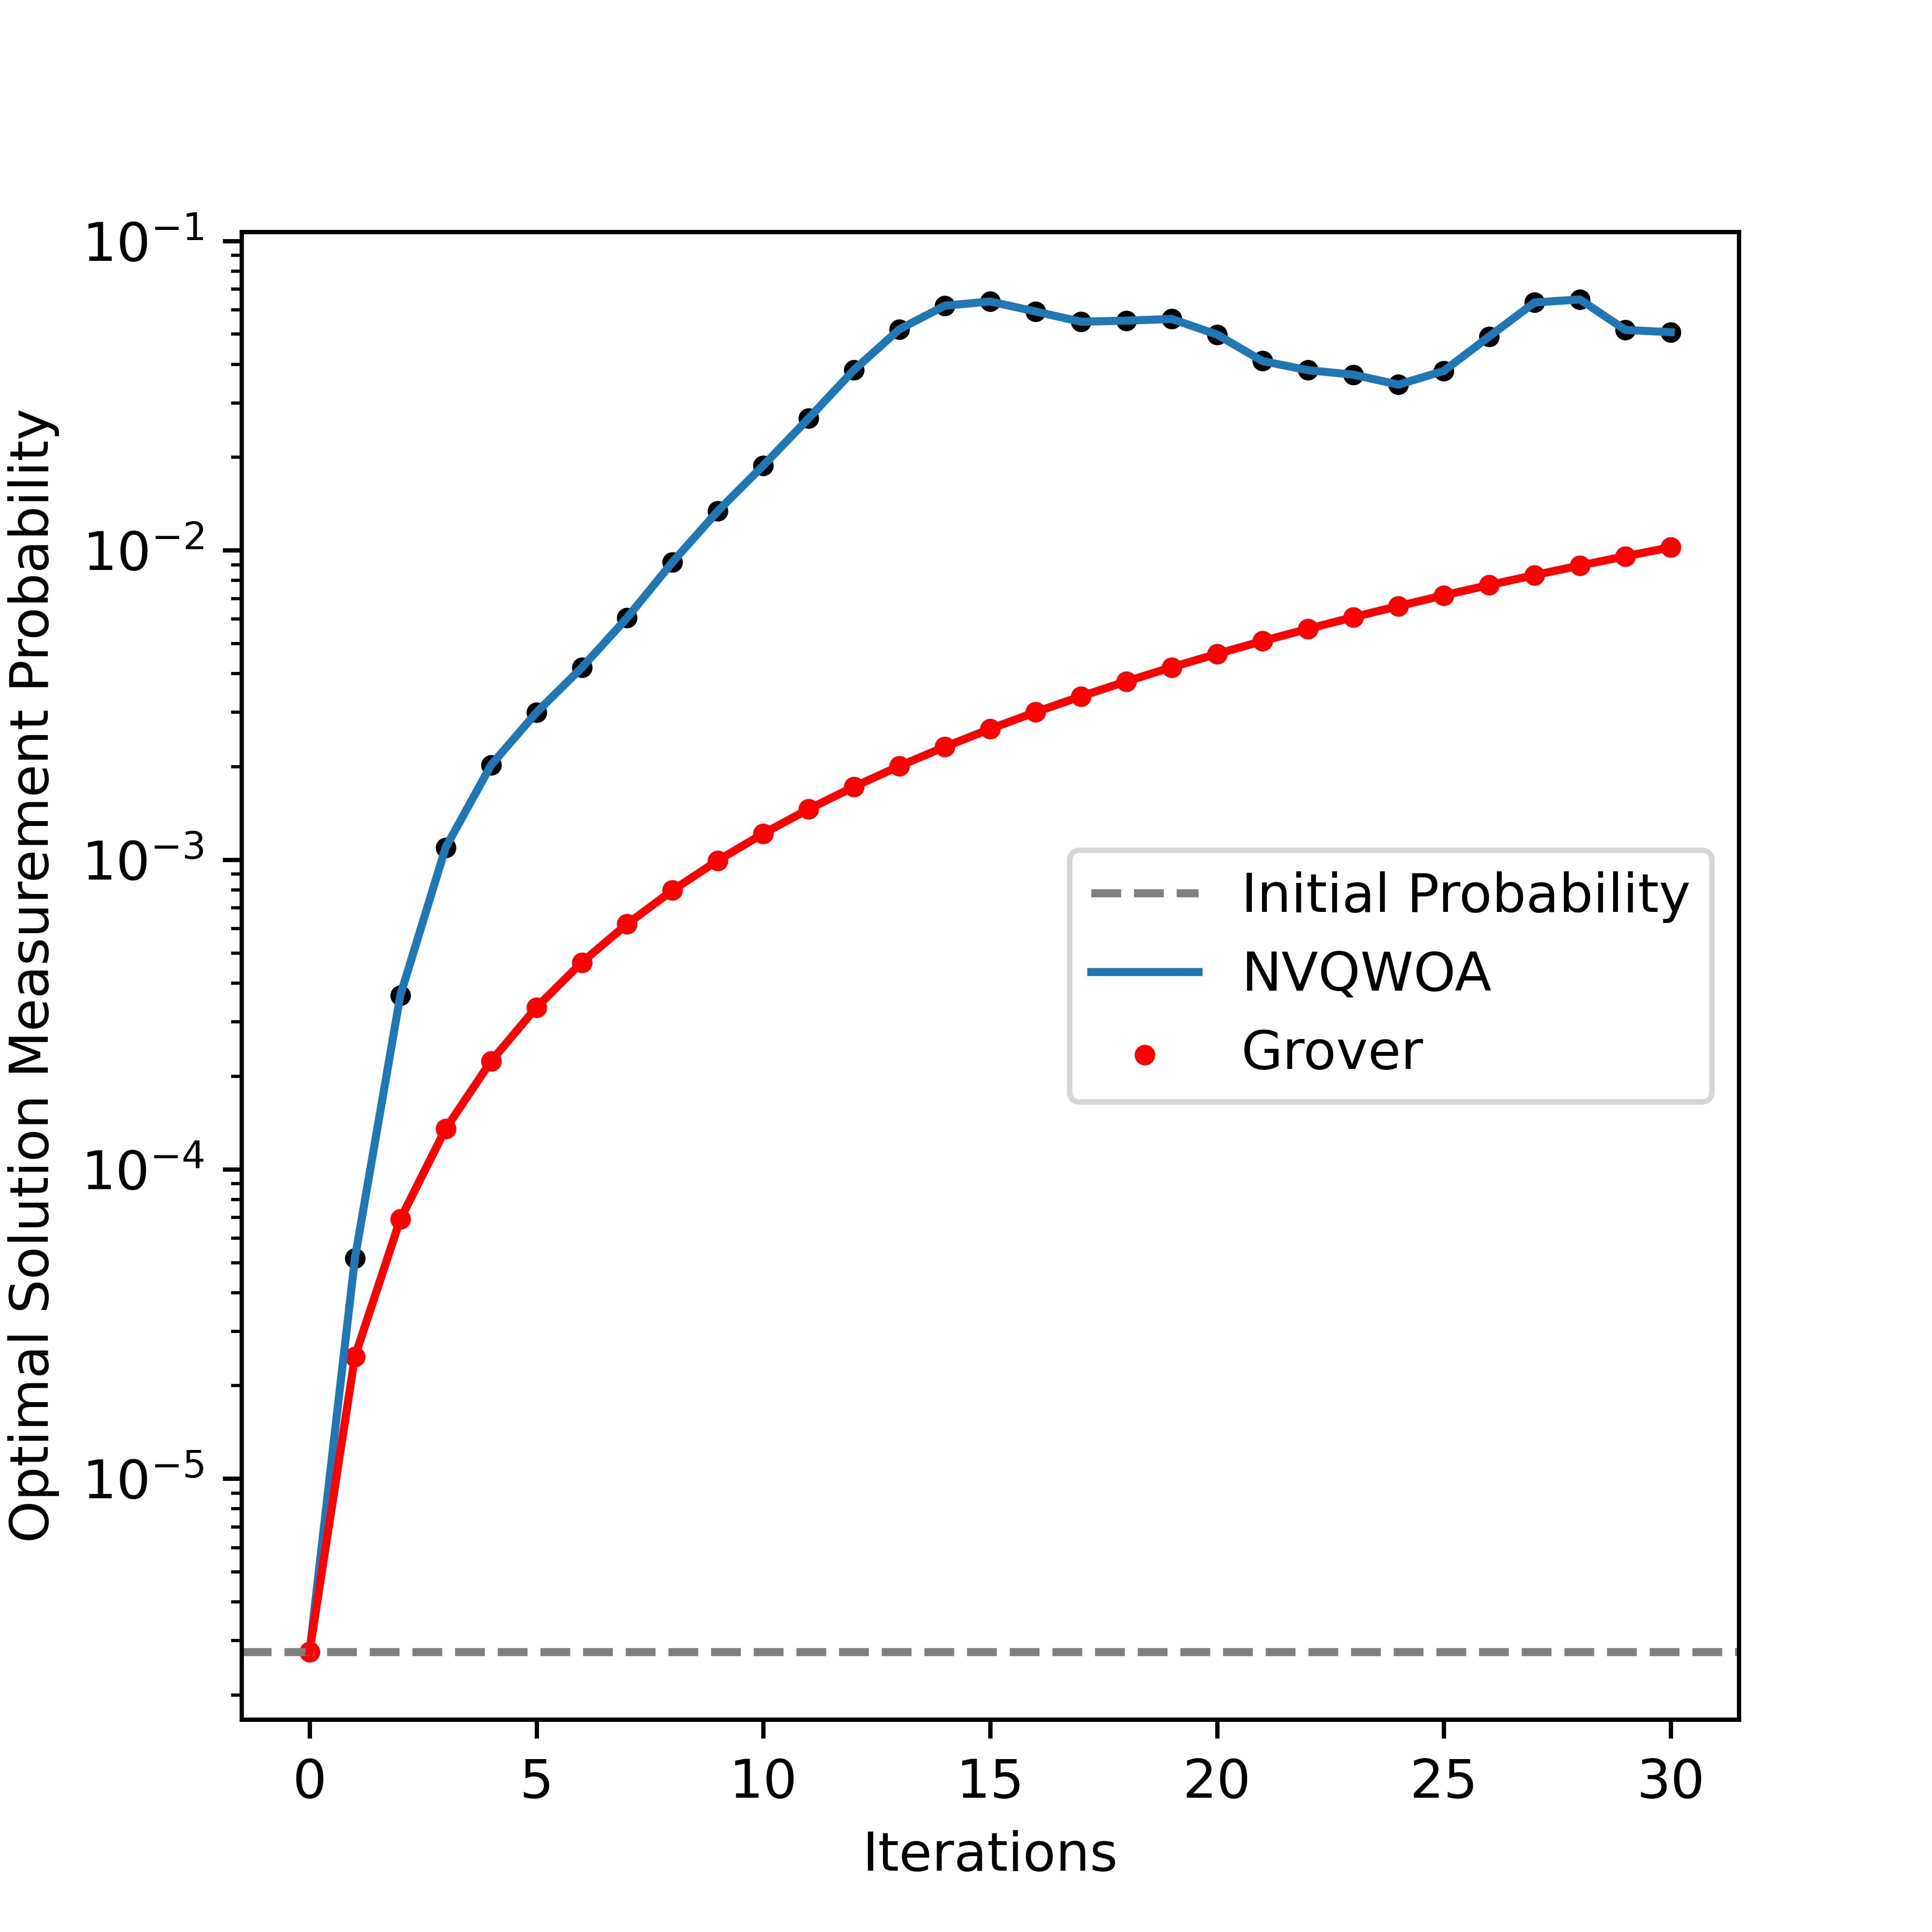
\includegraphics[width=\textwidth]{seed_2025_Log_Optimal_solution_probabilities_n=9_p=30_1.png}
\caption{ }
\label{fig:2025 log optimal}
\end{subfigure}
\hfill
\begin{subfigure}{0.45\textwidth}
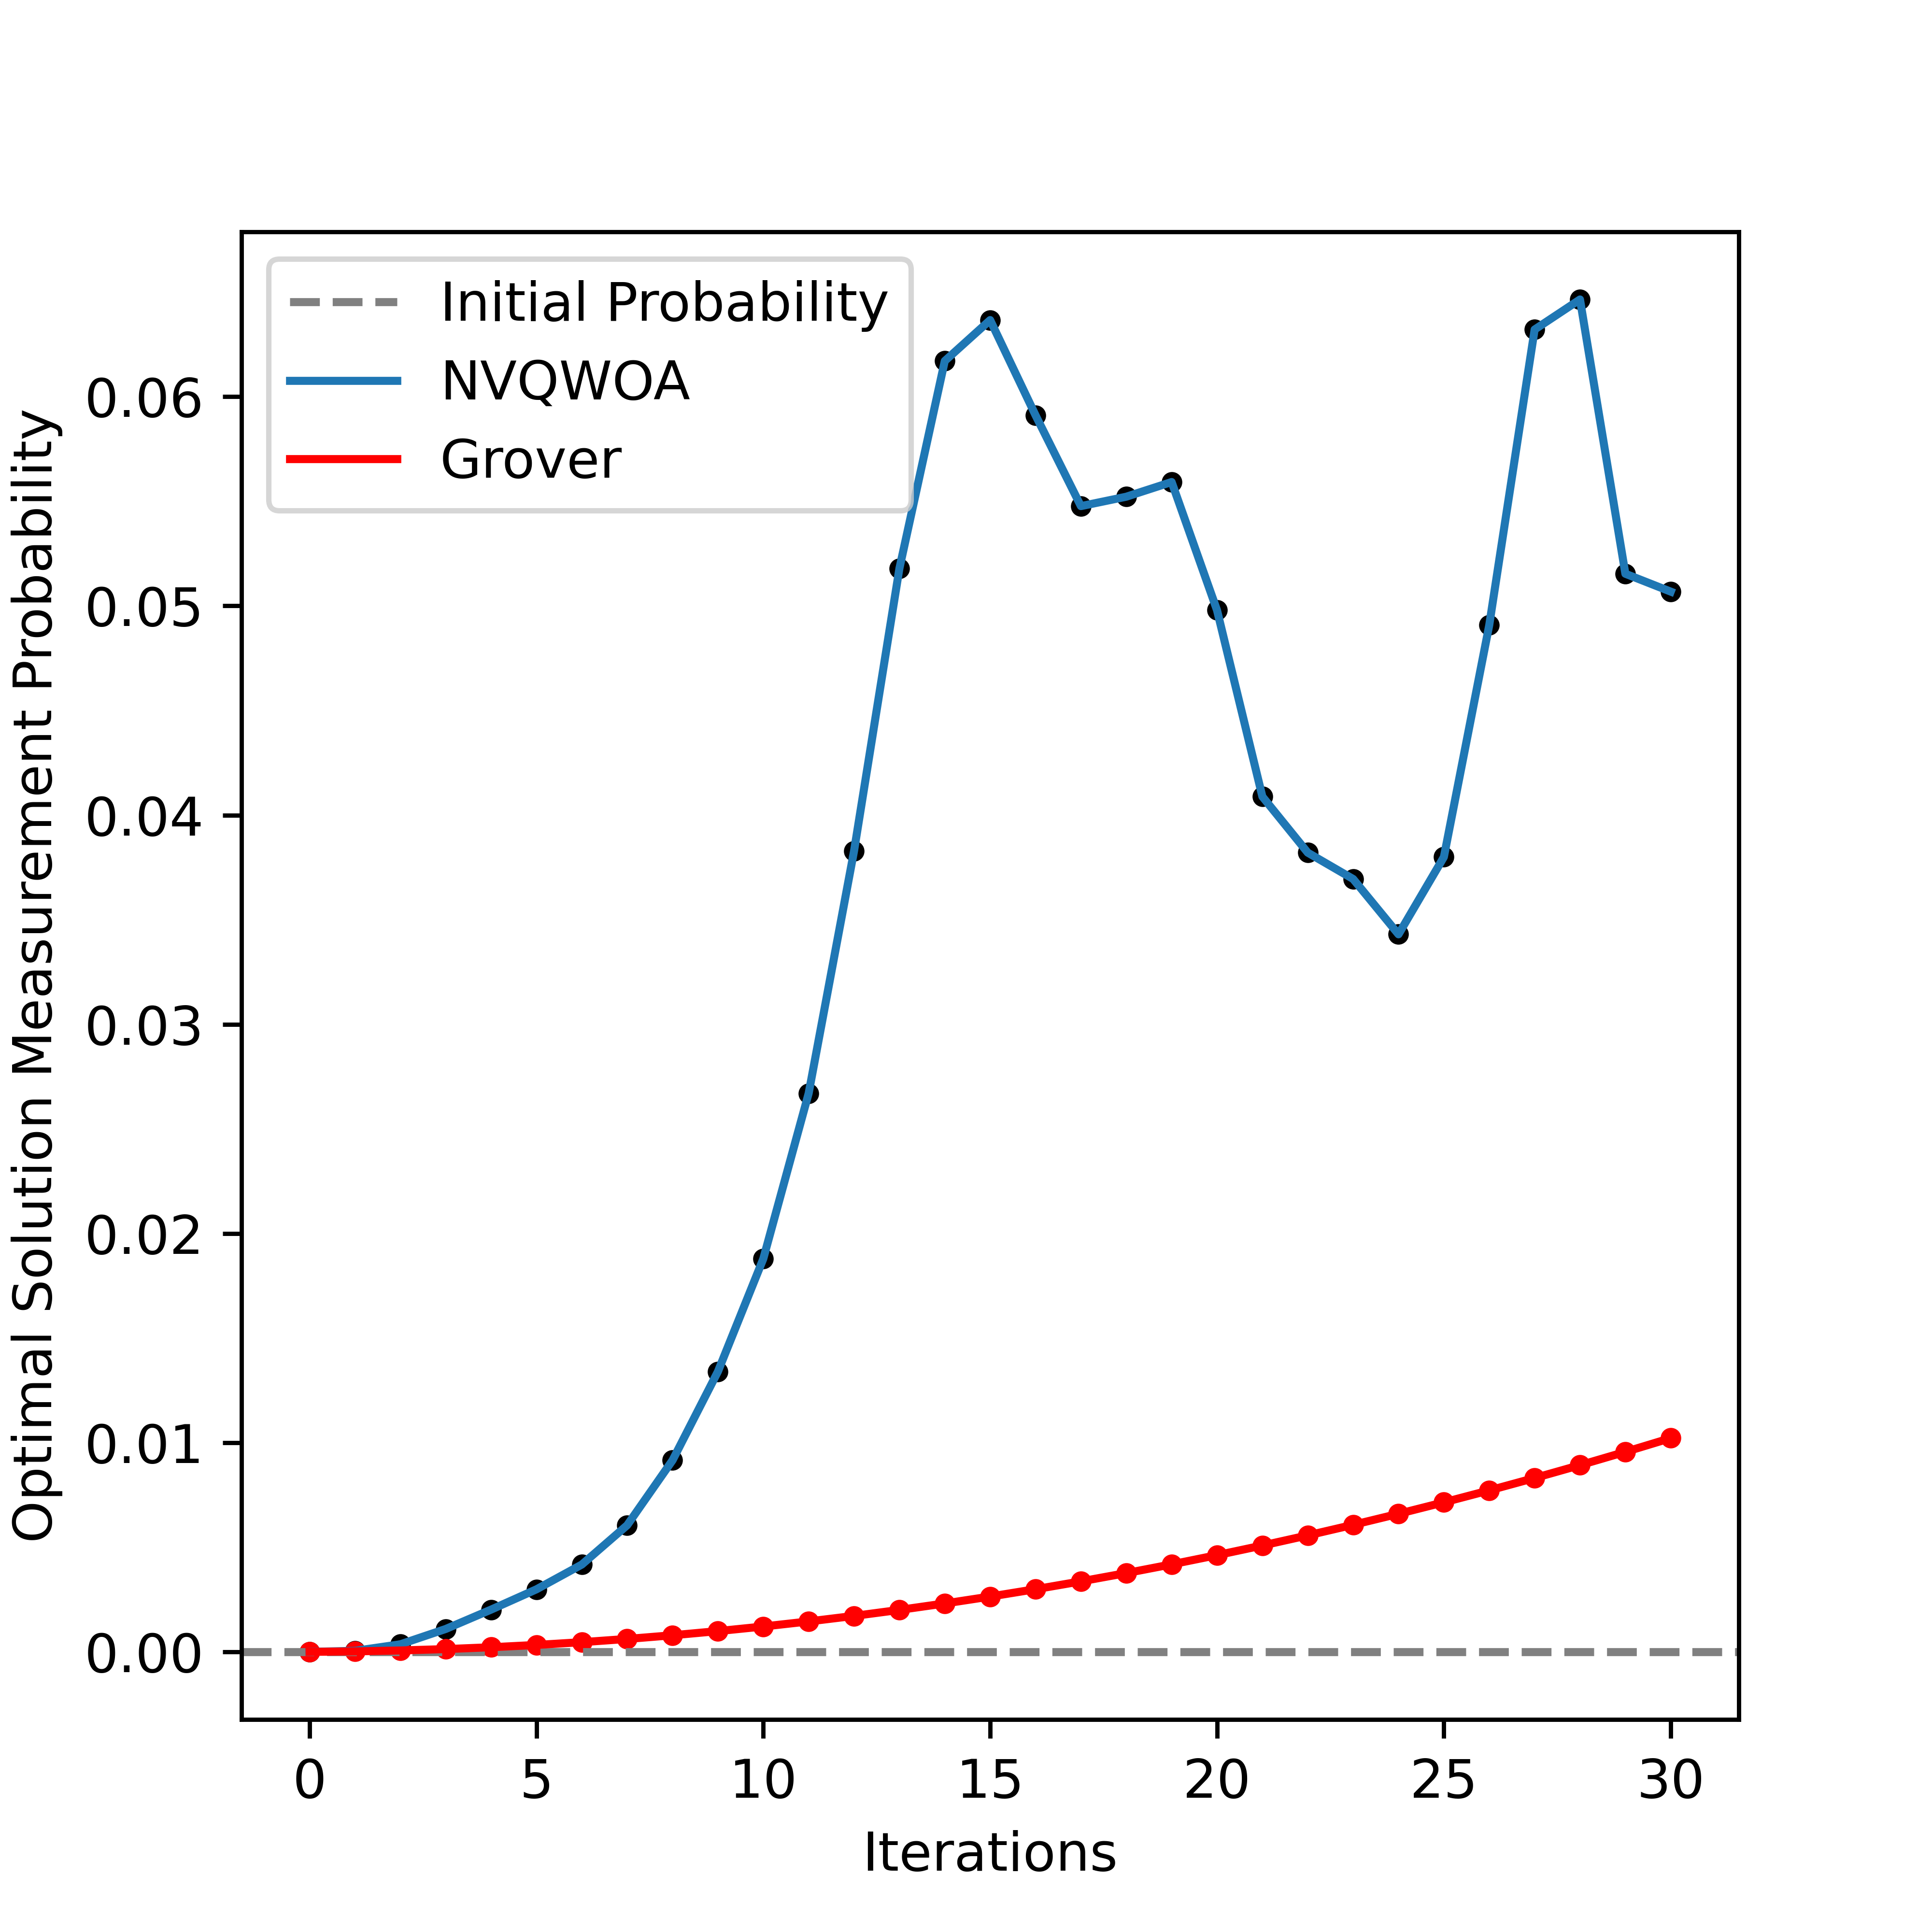
\includegraphics[width=\textwidth]{seed_2025_Optimal_solution_probabilities_n=9_p=30_1.png}
\caption{ }
\label{fig:2025 optimal}
\end{subfigure}
\caption{Simulation results for $p=30$ NVQWOA applied to seed 2025 and Grover's algorithm for an unstructured database of equivalent size. Probability of measuring the optimal solution at each iteration. (a) log scaled y-axis, (b) linear y-axis.}
\label{fig:2025 osp}
\end{figure}

\begin{figure}[htbp]
    \centering
    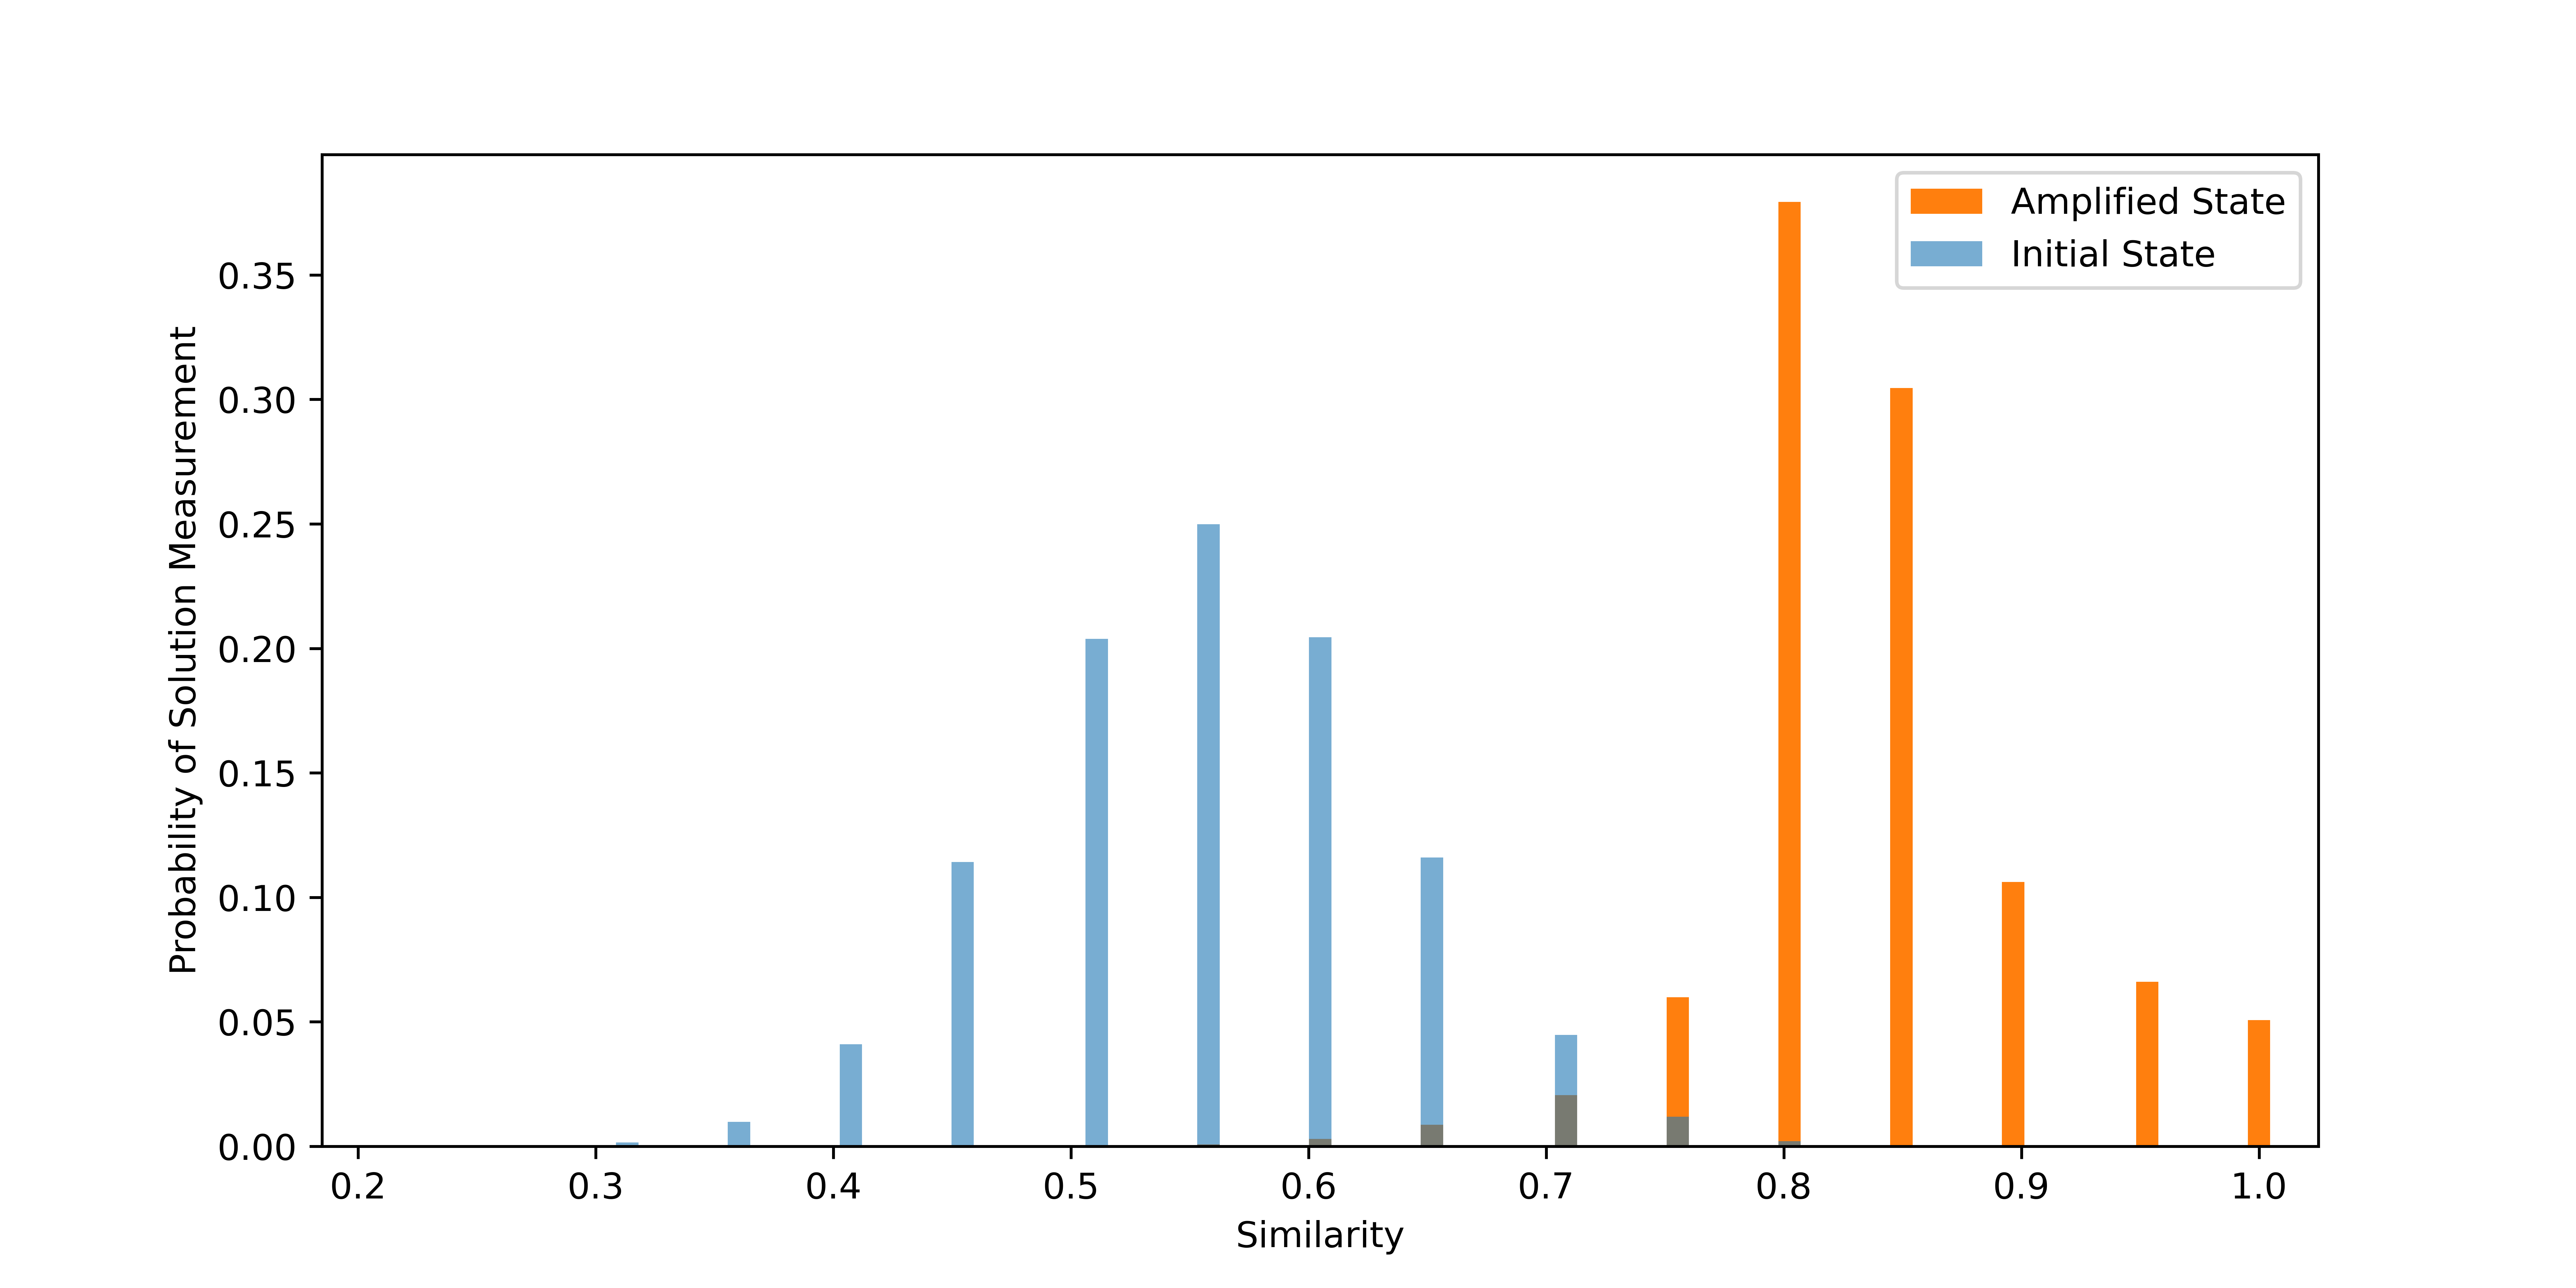
\includegraphics[width=\textwidth]{seed_2025_Objective_function_distributions_n=9_p=30_1.png}
    \caption{Simulation results for NVQWOA applied to seed 2025. Probability distributions for similarity as measured from the initial equal superposition state (blue) and the final amplified state (orange).}
    \label{fig:2025 similarity dist}
\end{figure}


Figures \ref{fig:2025 osp} and \ref{fig:2025 similarity dist} analyse the effect of the NVQWOA when applied to the graph $n=9$, seed$=2025$. From these results it is clear that probability amplitude has been channelled primarily into optimal and near-optimal solutions. 

In Figure \ref{fig:2025 osp}, the NVQWOA outperforms Grover's algorithm for an equivalent number of iterations. Since Grover's algorithm is optimal for searching an unstructured database \cite{grover_optimal}, this suggests the the NVQWOA is successfully using the structure of the problem (as embedded in the phase separation and mixing unitaries) to amplify the optimal solutions. Another feature of note is that after $p=15$ iterations, the OSP$=0.0636607501$ is at a maximum, and after this point, the OSP decreases with further iterations until it reaches 0.0342996063. The OSP appears to oscillate between those values, and ends on a value of 0.0506801642.

In Figure \ref{fig:2025 similarity dist}, the expected value for the similarity has increased from 0.556927 to 0.840676. The mode of the distribution has moved from a similarity score that had 90690 states to a similarity score with only 748 states. Even though the probability of measuring the optimal solution has increased, it is not the new mode of the probability distribution. This is because there is only 1 optimal solution, so even though the other solutions have less amplification applied to them, they greatly outnumber the optimal solution usually by two or three orders of magnitude. Therefore, any small amount of probability that they receive can sum up to be greater than the solution receiving the most amplification.

This is further verified in Figure \ref{fig:2025 av amp}. Solutions with similarity below 0.75 are attenuated by the NVQWOA, and solutions with similarity greater than 0.75 are amplified, with the amplification increasing exponentially with similarity. The amount of amplification that the optimal solution receives is greater than any other solution, with an amplification factor of 18391. The similarity score of the solutions with the most attenuation is 0.25925926, with an amplification factor of $3.73\times10^{-5}$. Interestingly, the solutions with the most attenuation are not those with the minimum similarity scores. The minimum quality solutions, which have a similarity of 0.20987654, received an average amplification of $3.33\times10^{-3}$, which is more amplification than was applied to any other solutions with similarity score less than 0.6. This reduction in attenuation is due to the mapping of qualities onto the unit circle as part of the algorithm. EXPAND ON THIS.

\begin{figure}[htbp]
    \centering
    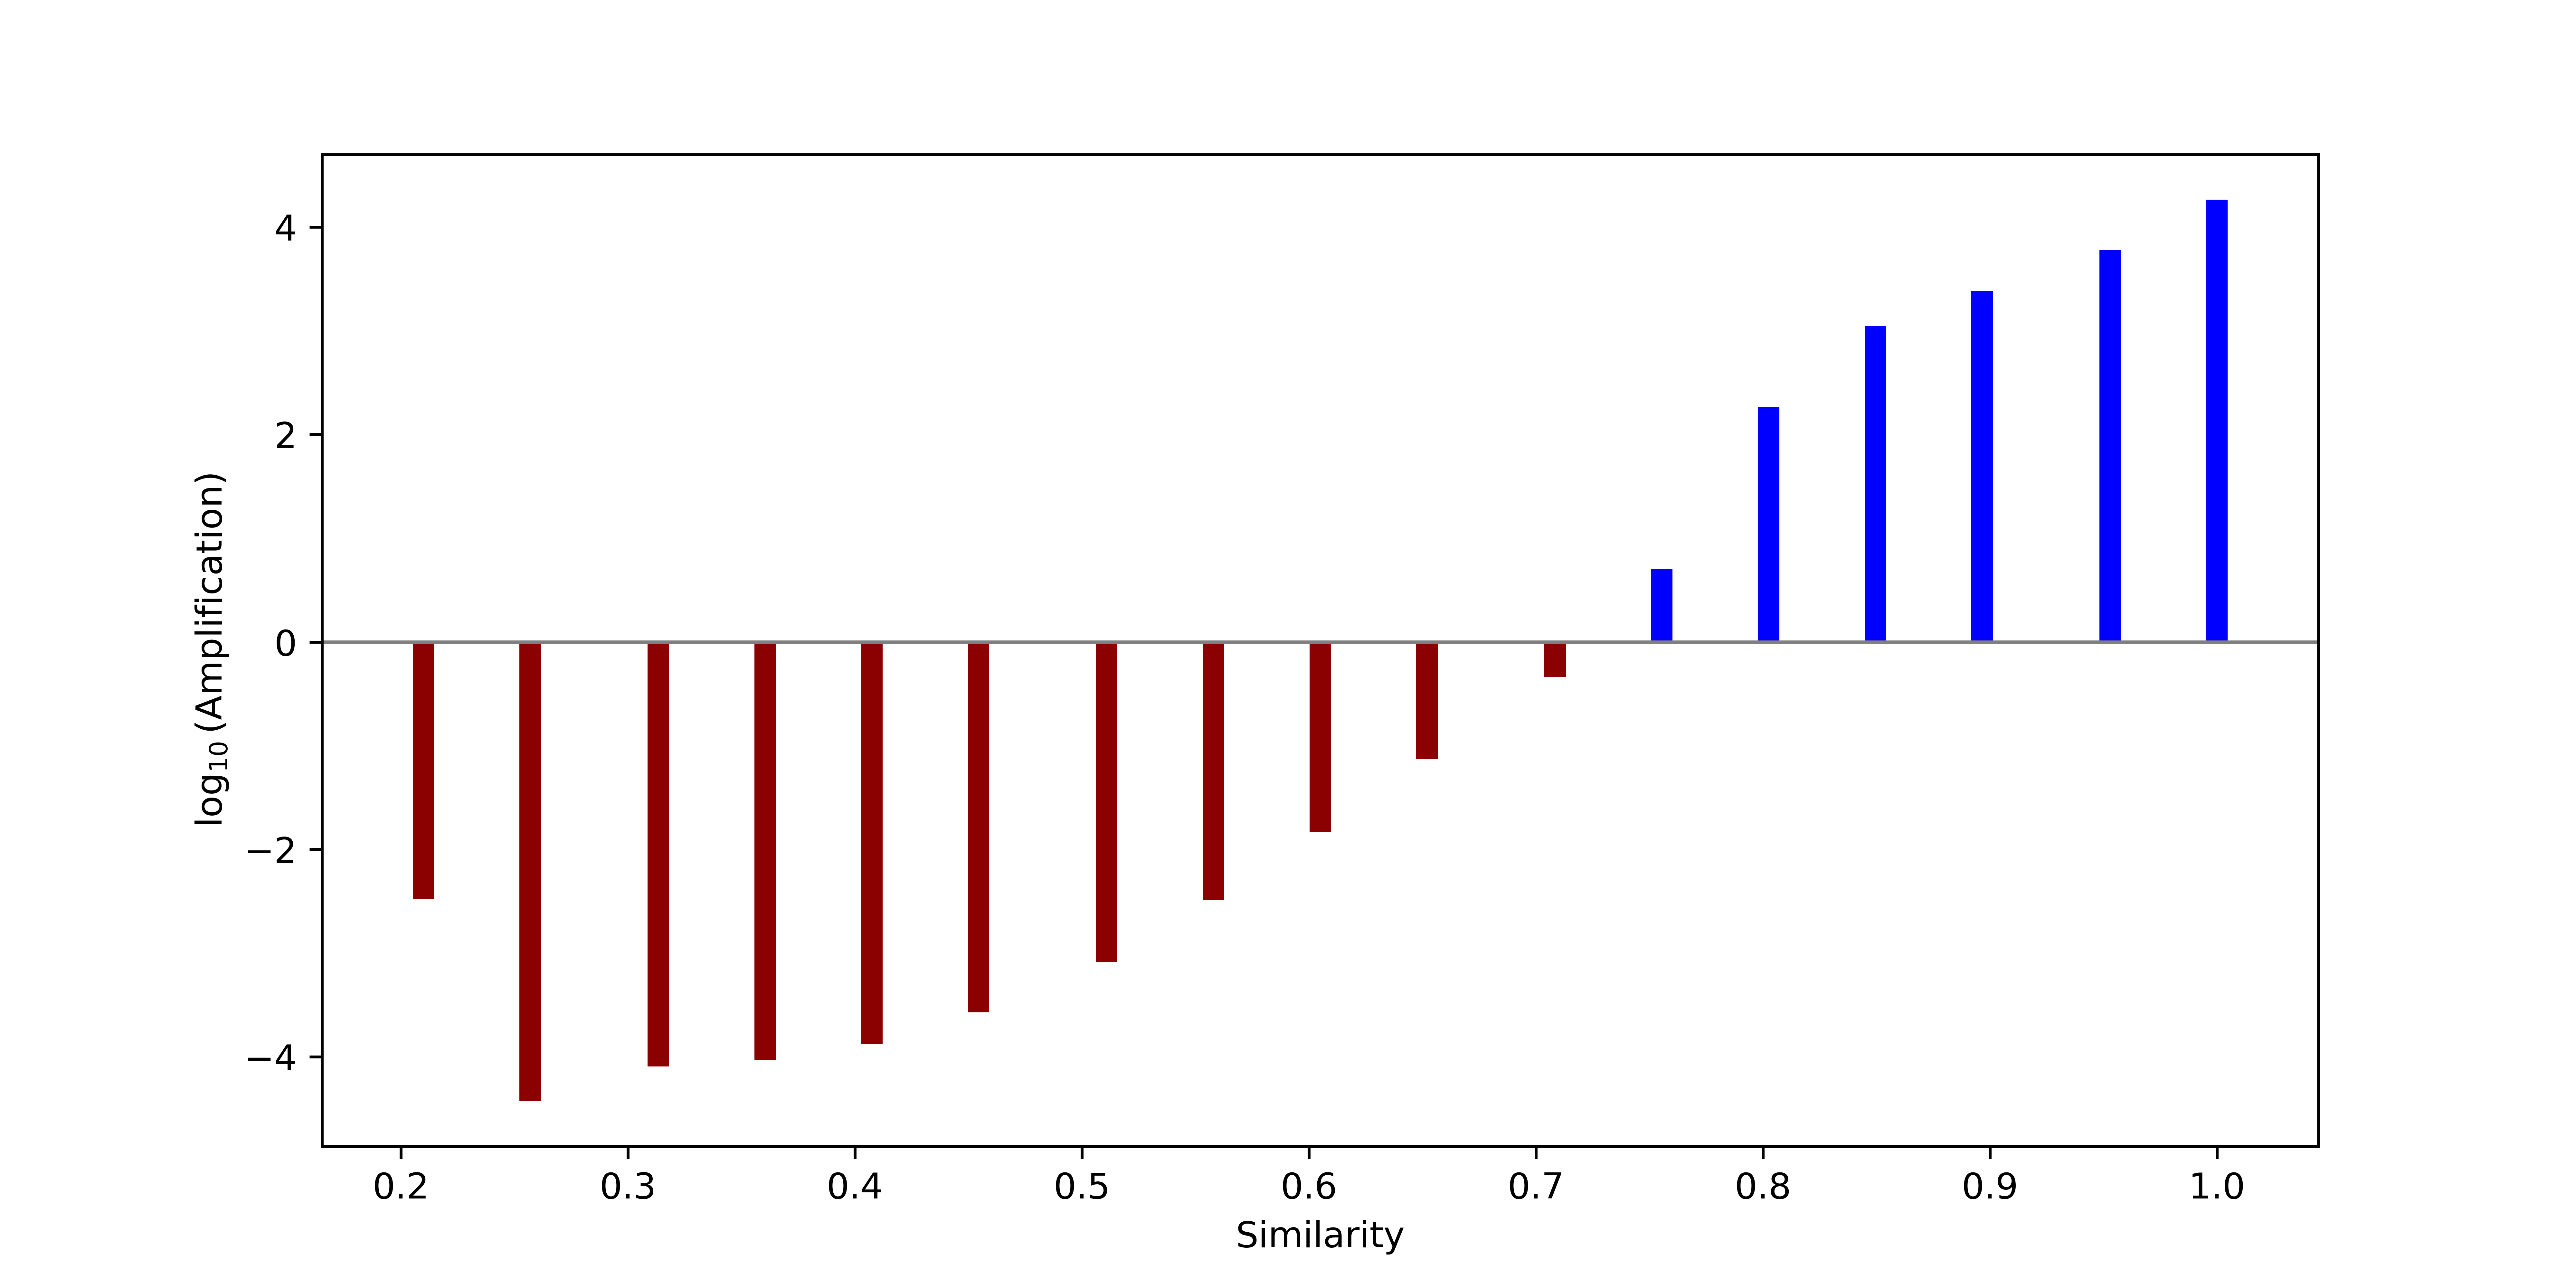
\includegraphics[width=\textwidth]{seed_2025_Log_average_amplification_n=9_p=30_1.png}
    \caption{Simulation results for NVQWOA applied to seed 2025. Logarithmic scale solution amplification as a function of solution similarity.}
    \label{fig:2025 av amp}
\end{figure}

\begin{figure}[htbp]
\centering
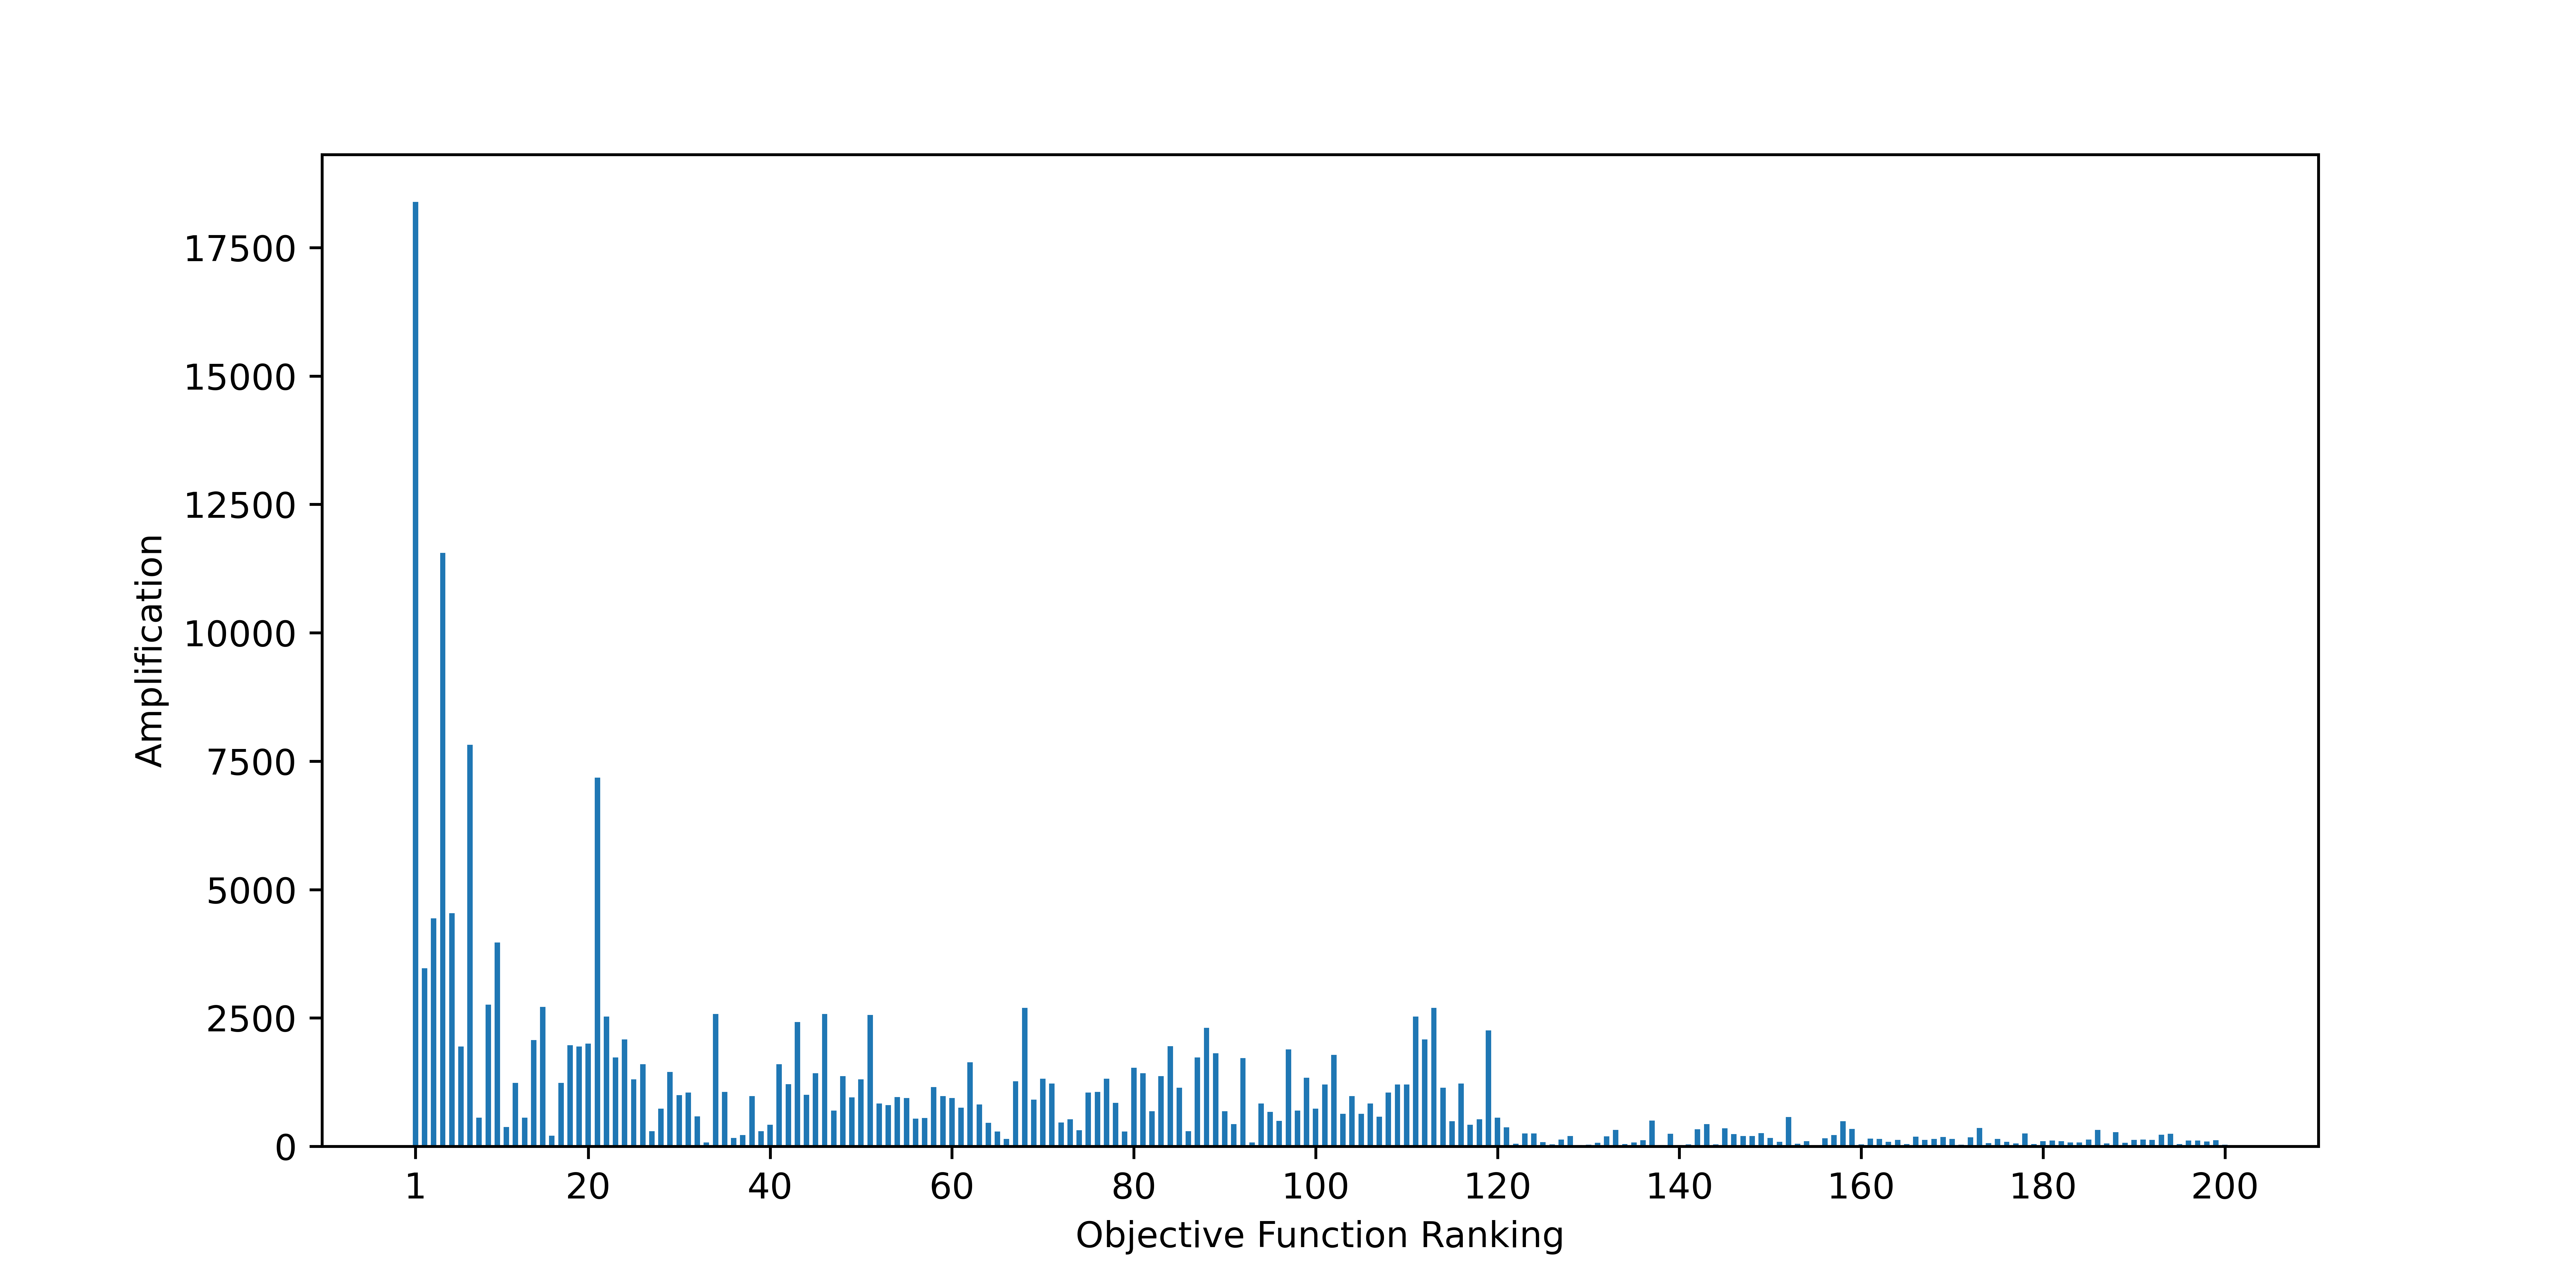
\includegraphics[width=\textwidth]{seed_2025_Top_200_amplifications_n=9_p=30_1.png}
\caption{Simulation results for NVQWOA applied to seed 2025. Amplification applied to the best 200 solutions.}
\end{figure}



\section{Multiple Graph Analysis}
The next phase in the analysis was to perform simulations on many different graphs and observe how the algorithm performs in the average case. For these simulations, the number of iterations was decreased to $p=10$, and hyperparameter optimisation was used to find suitable hyperparameters for each problem. As discussed in section \ref{sec:parameters}, the hyperparameter optimisation objective functions used were expected value (EV), optimal solution probability (OSP), and conditional value at risk (CVaR).

\subsection{Algorithm Behaviour and Amplification}

To expand on the results from the previous section, probability distributions for the similarities were analysed. Figures \ref{fig:similarity dist} and \ref{fig:similarity log dist} show the average probability distributions over the possible similarity scores, using a linear probability scale for Figure \ref{fig:similarity dist} and a log probability scale for \ref{fig:similarity log dist}. After amplification, the distributions are skewed towards higher-similarity solutions compared to the initial distribution. In the distributions representing the average final state for OSP, the modes are not shifted as much as the modes for EV or CVaR. This is because CVaR and EV can be improved by shifting up the mode of the probability distribution, even if the optimal solution probability decreases.

\begin{figure}[htbp]
    \centering
    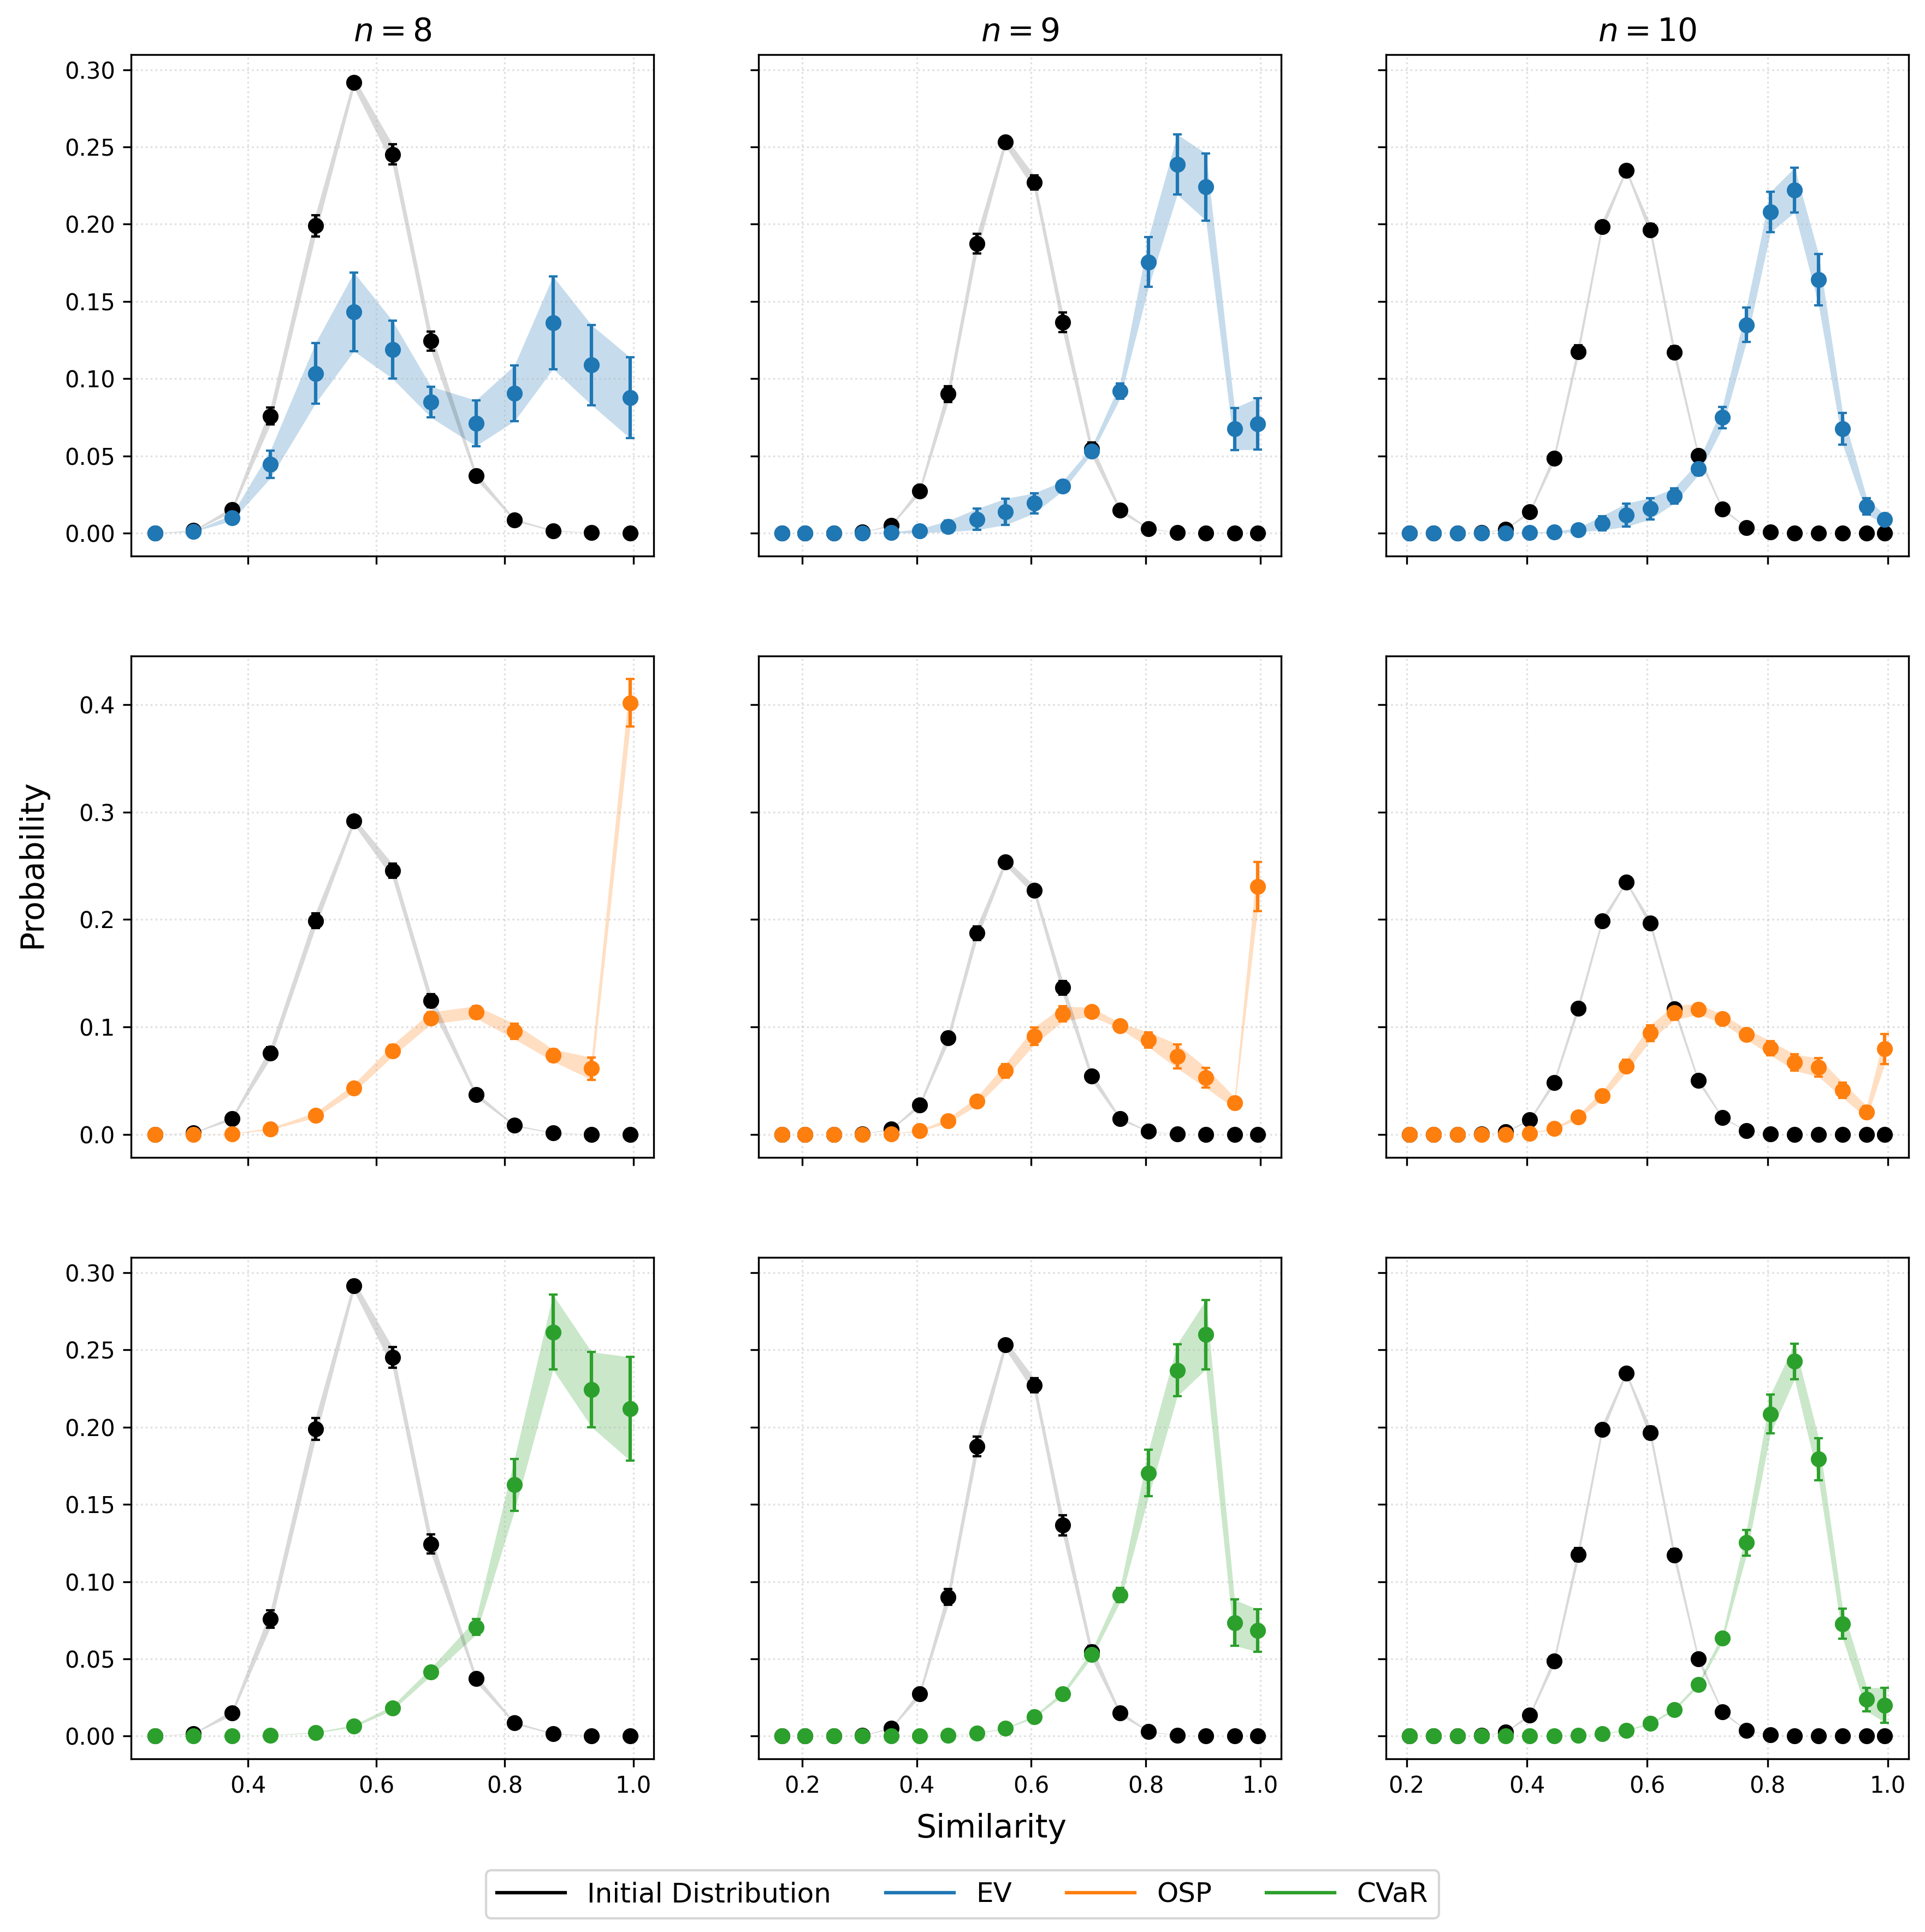
\includegraphics[width=\textwidth]{similarity_distributions_multiple.png} 
    \caption{Probability distributions for similarity as measured from the initial equal superposition state (black) and the final amplified state.Average simulation results for NVQWOA applied to 30 graphs at (left) $n=8$, (center) $n=9$, (right) $n=10$. (Top) hyperparameters optimised for EV. (Middle) hyperparameters optimised for OSP. (Bottom) hyperparameters optimised for CVaR.}
    \label{fig:similarity dist}
\end{figure}

\begin{figure}[htbp]
    \centering
    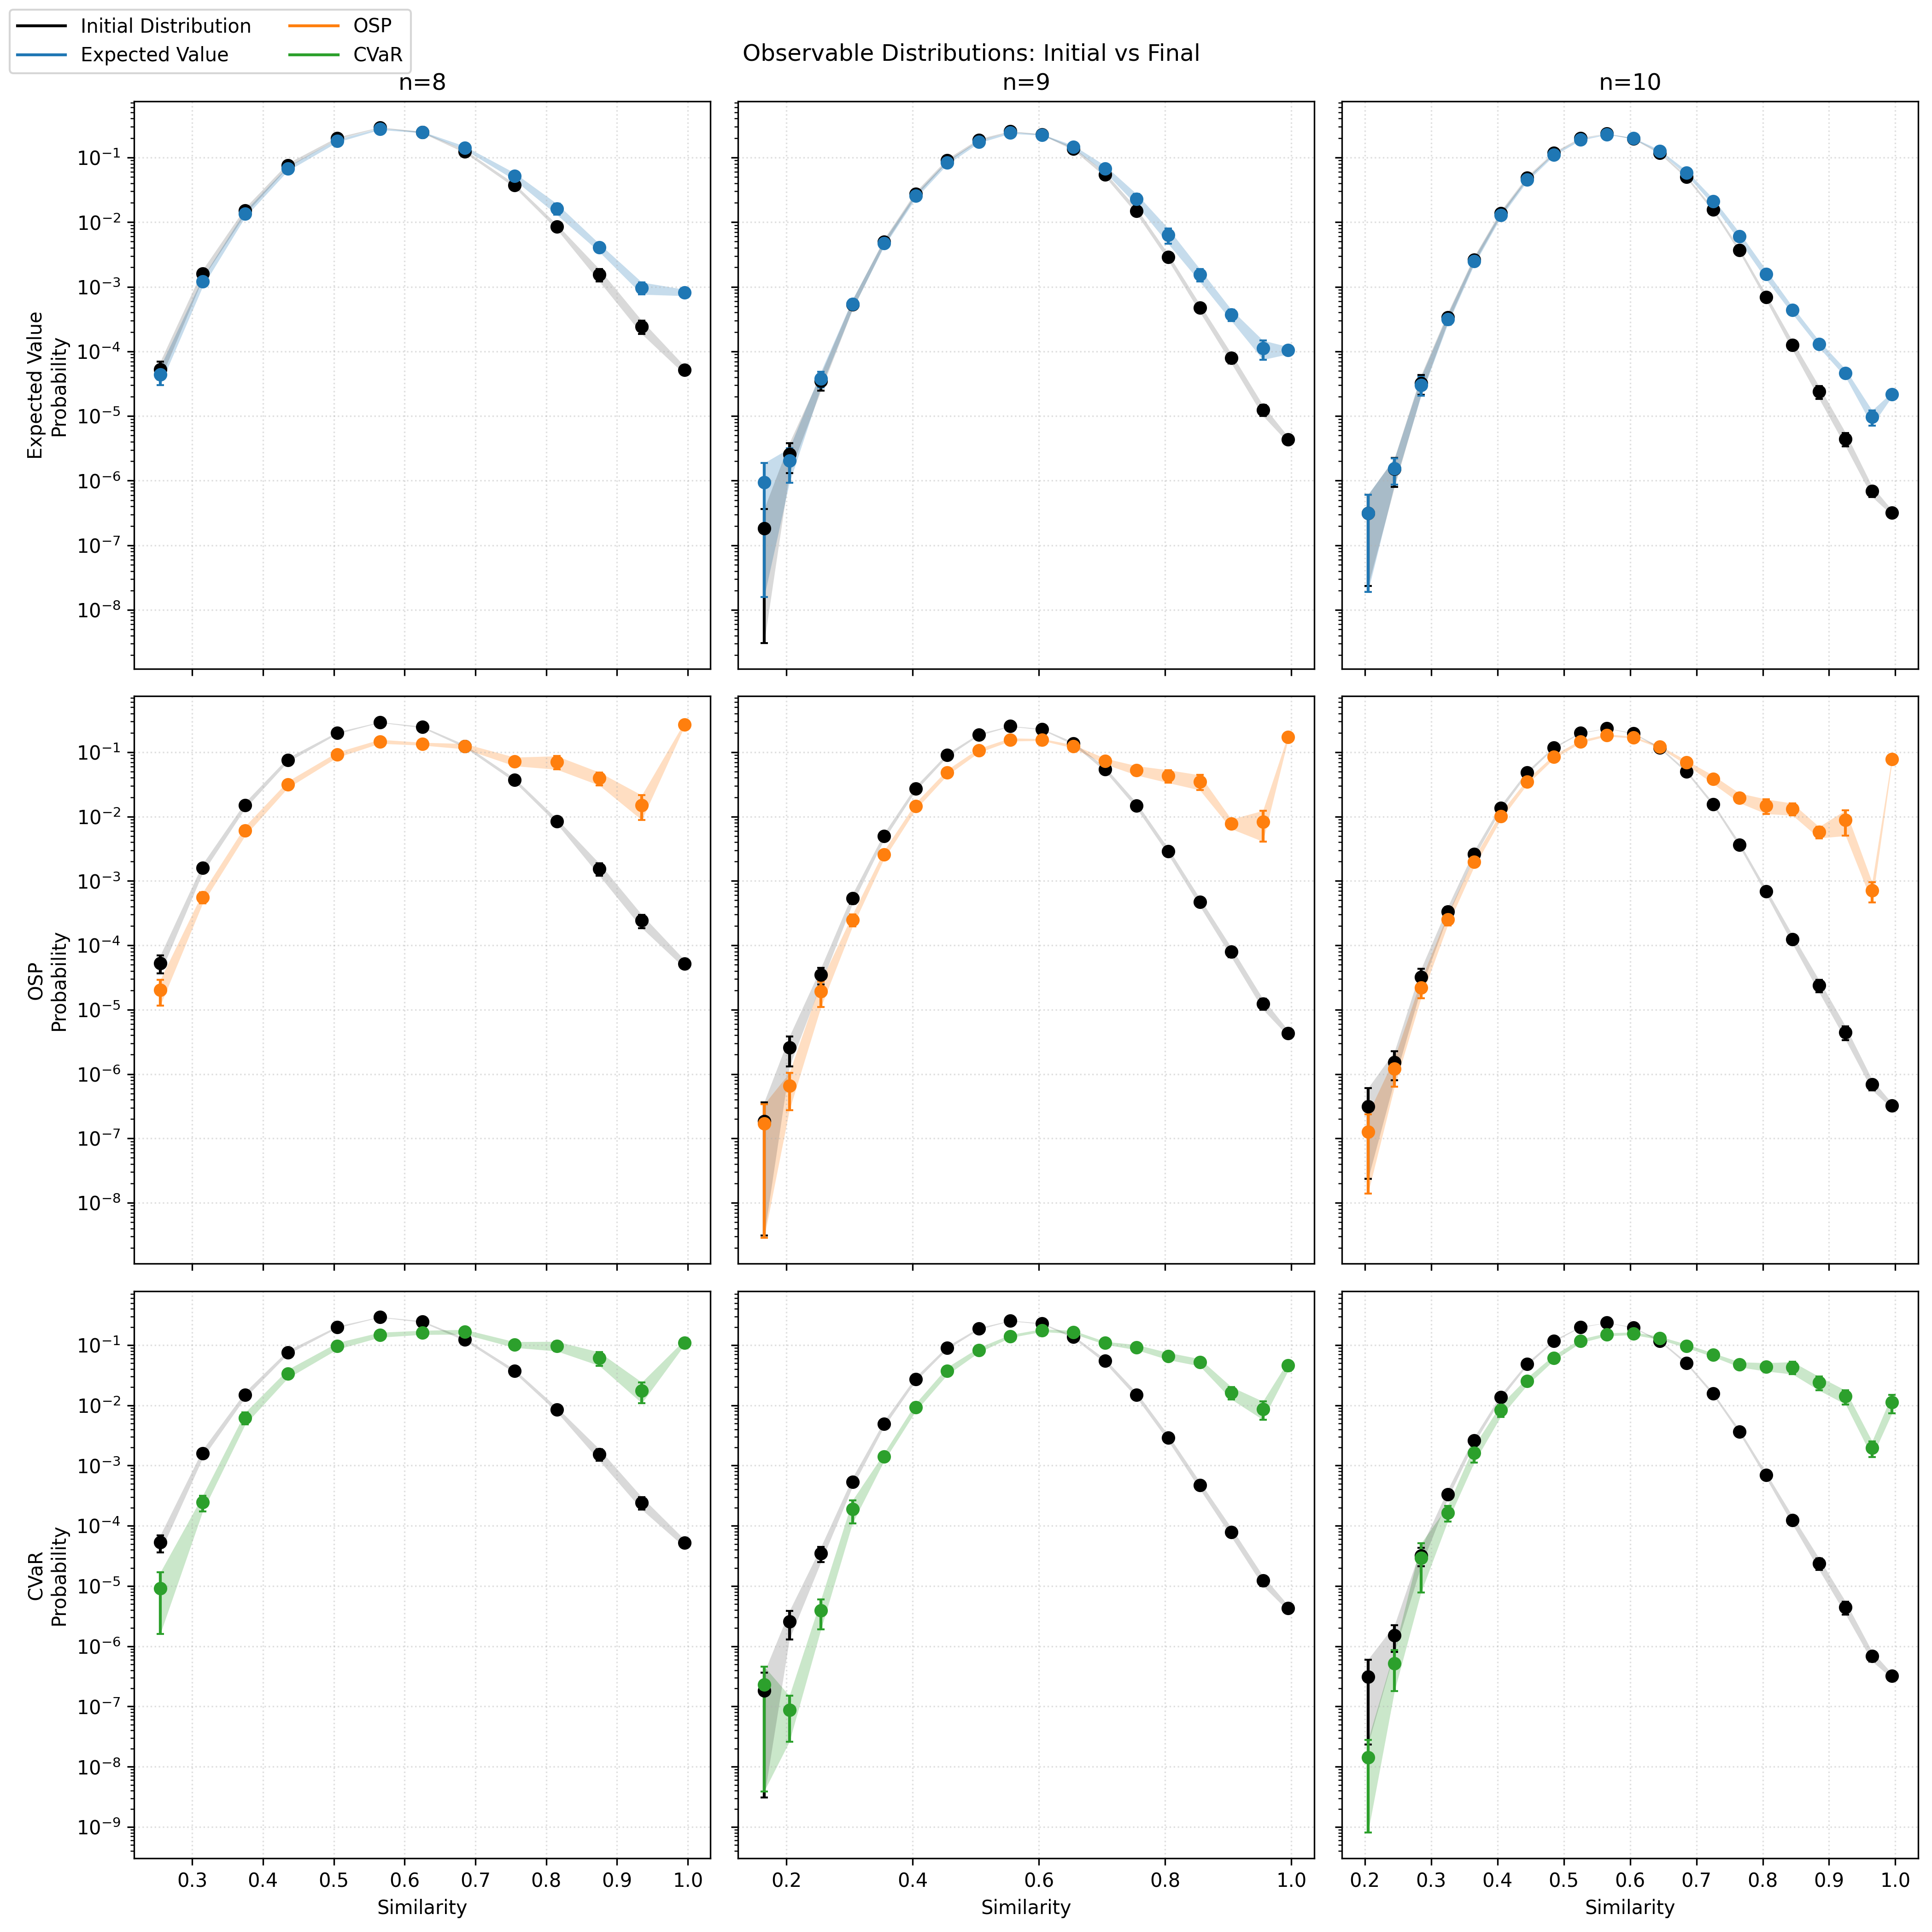
\includegraphics[width=\textwidth]{log_similarity_distributions_multiple.png} 
    \caption{Depicts the same distributions as Fig \ref{fig:similarity dist} with a logarithmic y-axis.}
    \label{fig:similarity log dist}
\end{figure}

Unexpectedly, it appears that for some seeds at $n=8$, optimising the hyperparameters for EV did not amplify the distribution at all. Rather disquieting. find an explanation for this.

\begin{figure}[htbp]
    \centering
    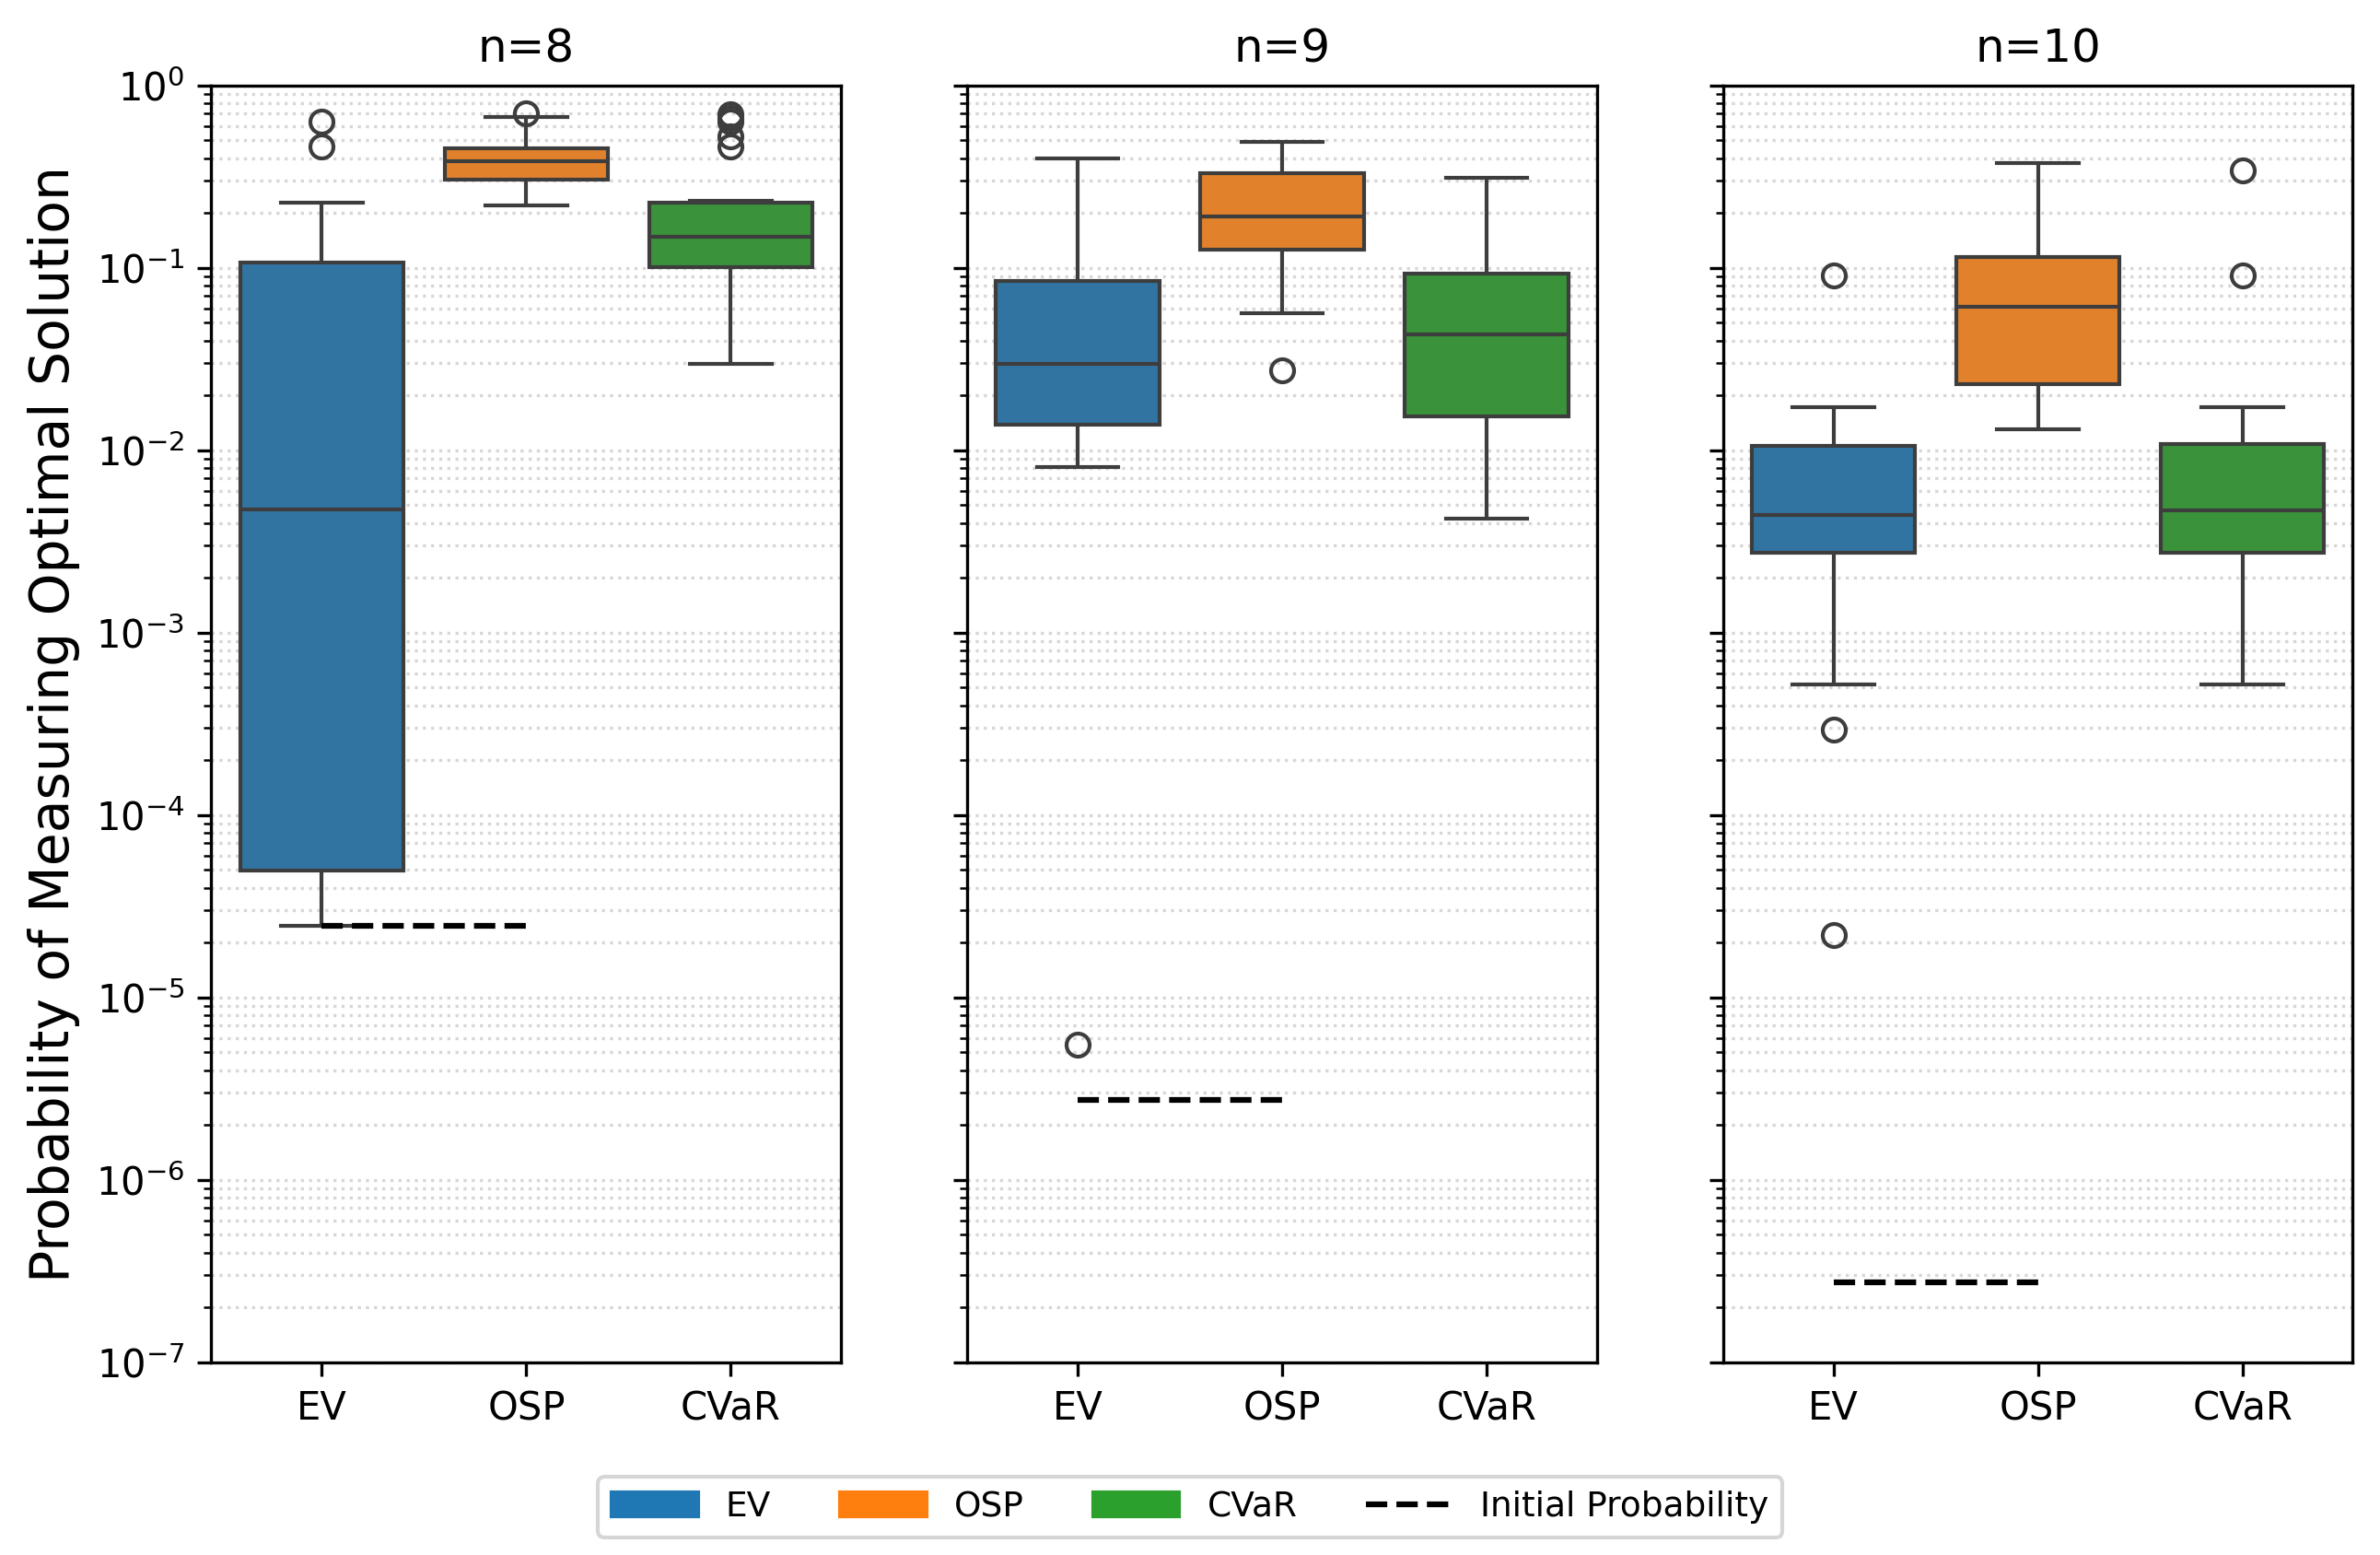
\includegraphics[width=\textwidth]{OSP_boxplot_multiple.png} 
    \caption{Simulation results of the NVQWOA applied to 30 graphs at (left)$n=8$, (center) $n=9$, (right) $n=10$. Boxplots represent the distribution in probability to measure the optimal solution.}
    \label{fig:osp}
\end{figure}

It is evident in Figure \ref{fig:osp} that the NVQWOA performs well in the average case to increase the probability of measuring the optimal solution. Additionally, comparing the fixed hyperparameter from the previous section to the optimised hyperparameters in the equivalent $n=9$ problem set here, we see that the final optimal solution probability has increased on average from 0.06366 to 0.23 for OSP, and 0.07 for EV and CVaR. However, given that the final optimal solution probability can vary over several orders of magnitude, whether hyperparameter optimisation assists in directly measuring the optimal solution appears to be in doubt.

\subsection{Distance Analysis}
We next analysed the distance between each solution and the optimal solution(s) to determine the degree to which amplification favours solutions close to the optimum in the solution space. The measures of distance used were Hamming distance and subshell distance, described in section \ref{sec:solution distance}.

As shown in Figure \ref{fig:ham improvement}, the mean Hamming distance decreased significantly after amplification, with X and Y and Z as the average reductions.
\begin{figure}[htbp]
    \centering
    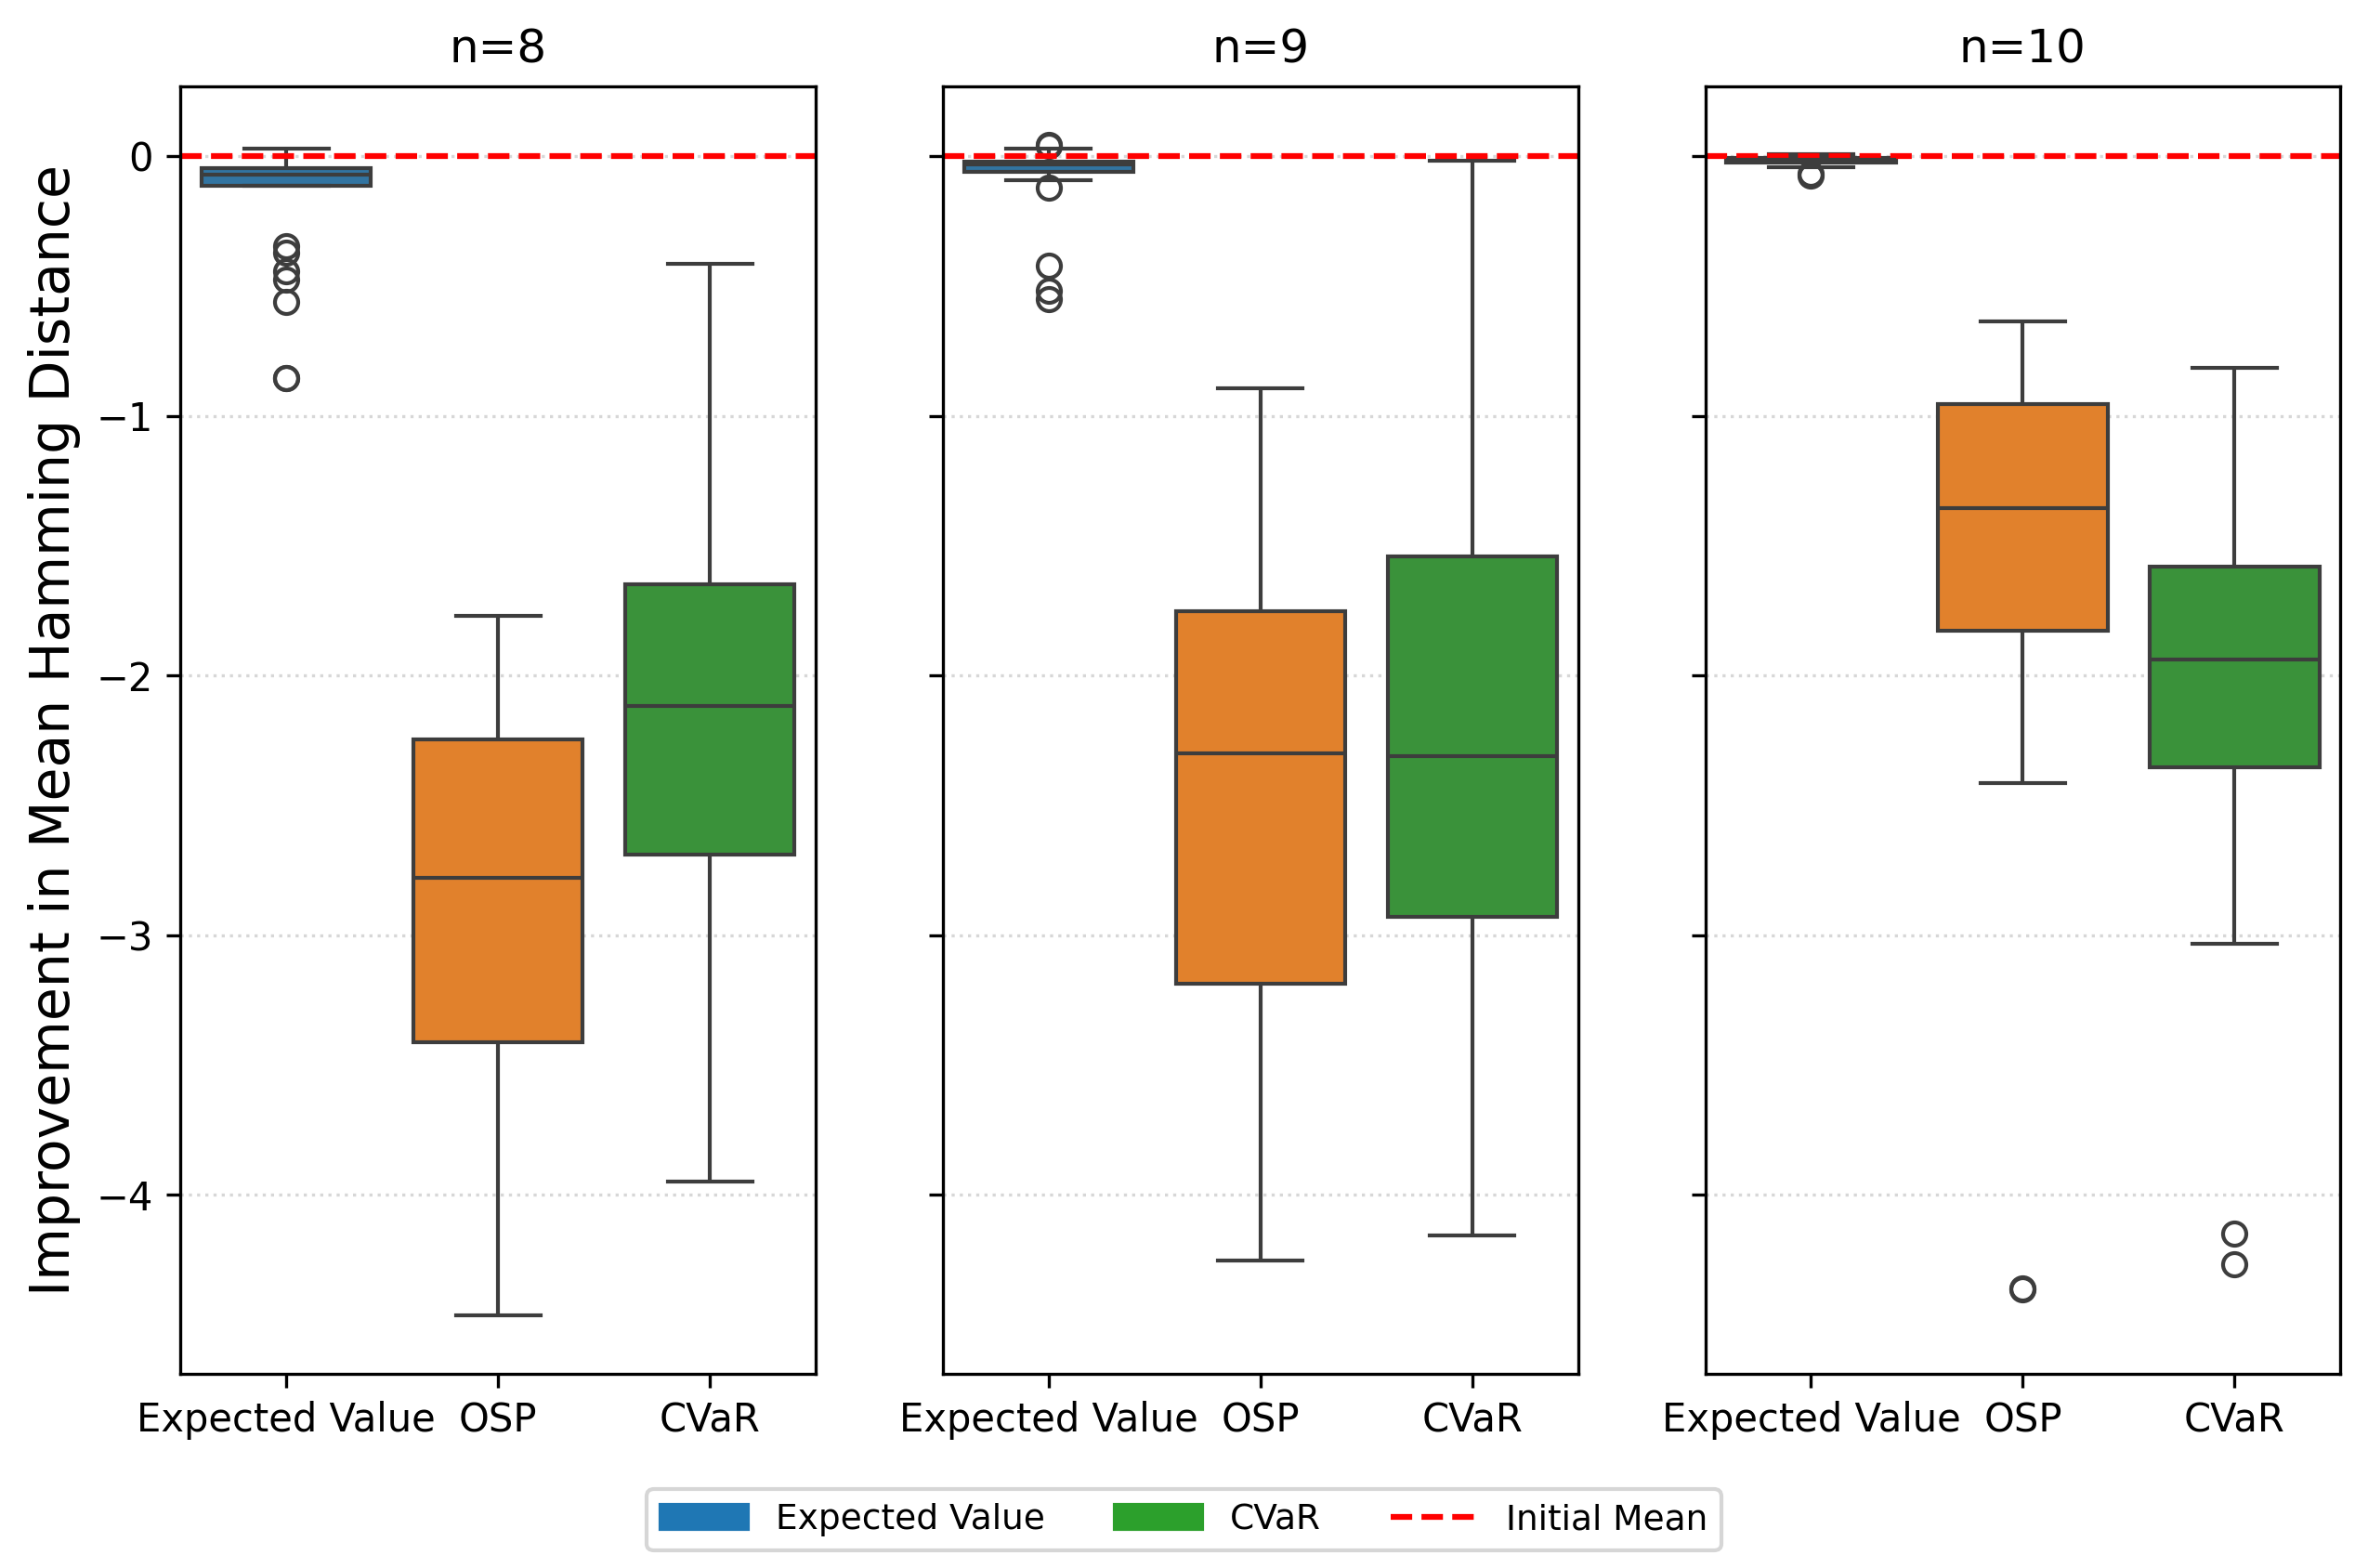
\includegraphics[width=\textwidth]{hamming_improvement_boxplot_multiple.png}
    \caption{Simulation results of the NVQWOA applied to 30 graphs at (left)$n=8$, (center) $n=9$, (right) $n=10$. Boxplots representing the distribution of improvements in mean Hamming distance. The Initial Mean (red)}
    \label{fig:ham improvement}
\end{figure}

Figure \ref{fig:amp vs ham} shows how much amplification was applied to each solution based on their Hamming distance. The optimal solutions received average amplifications of X,Y and Z.
\begin{figure}[htbp]
    \centering
    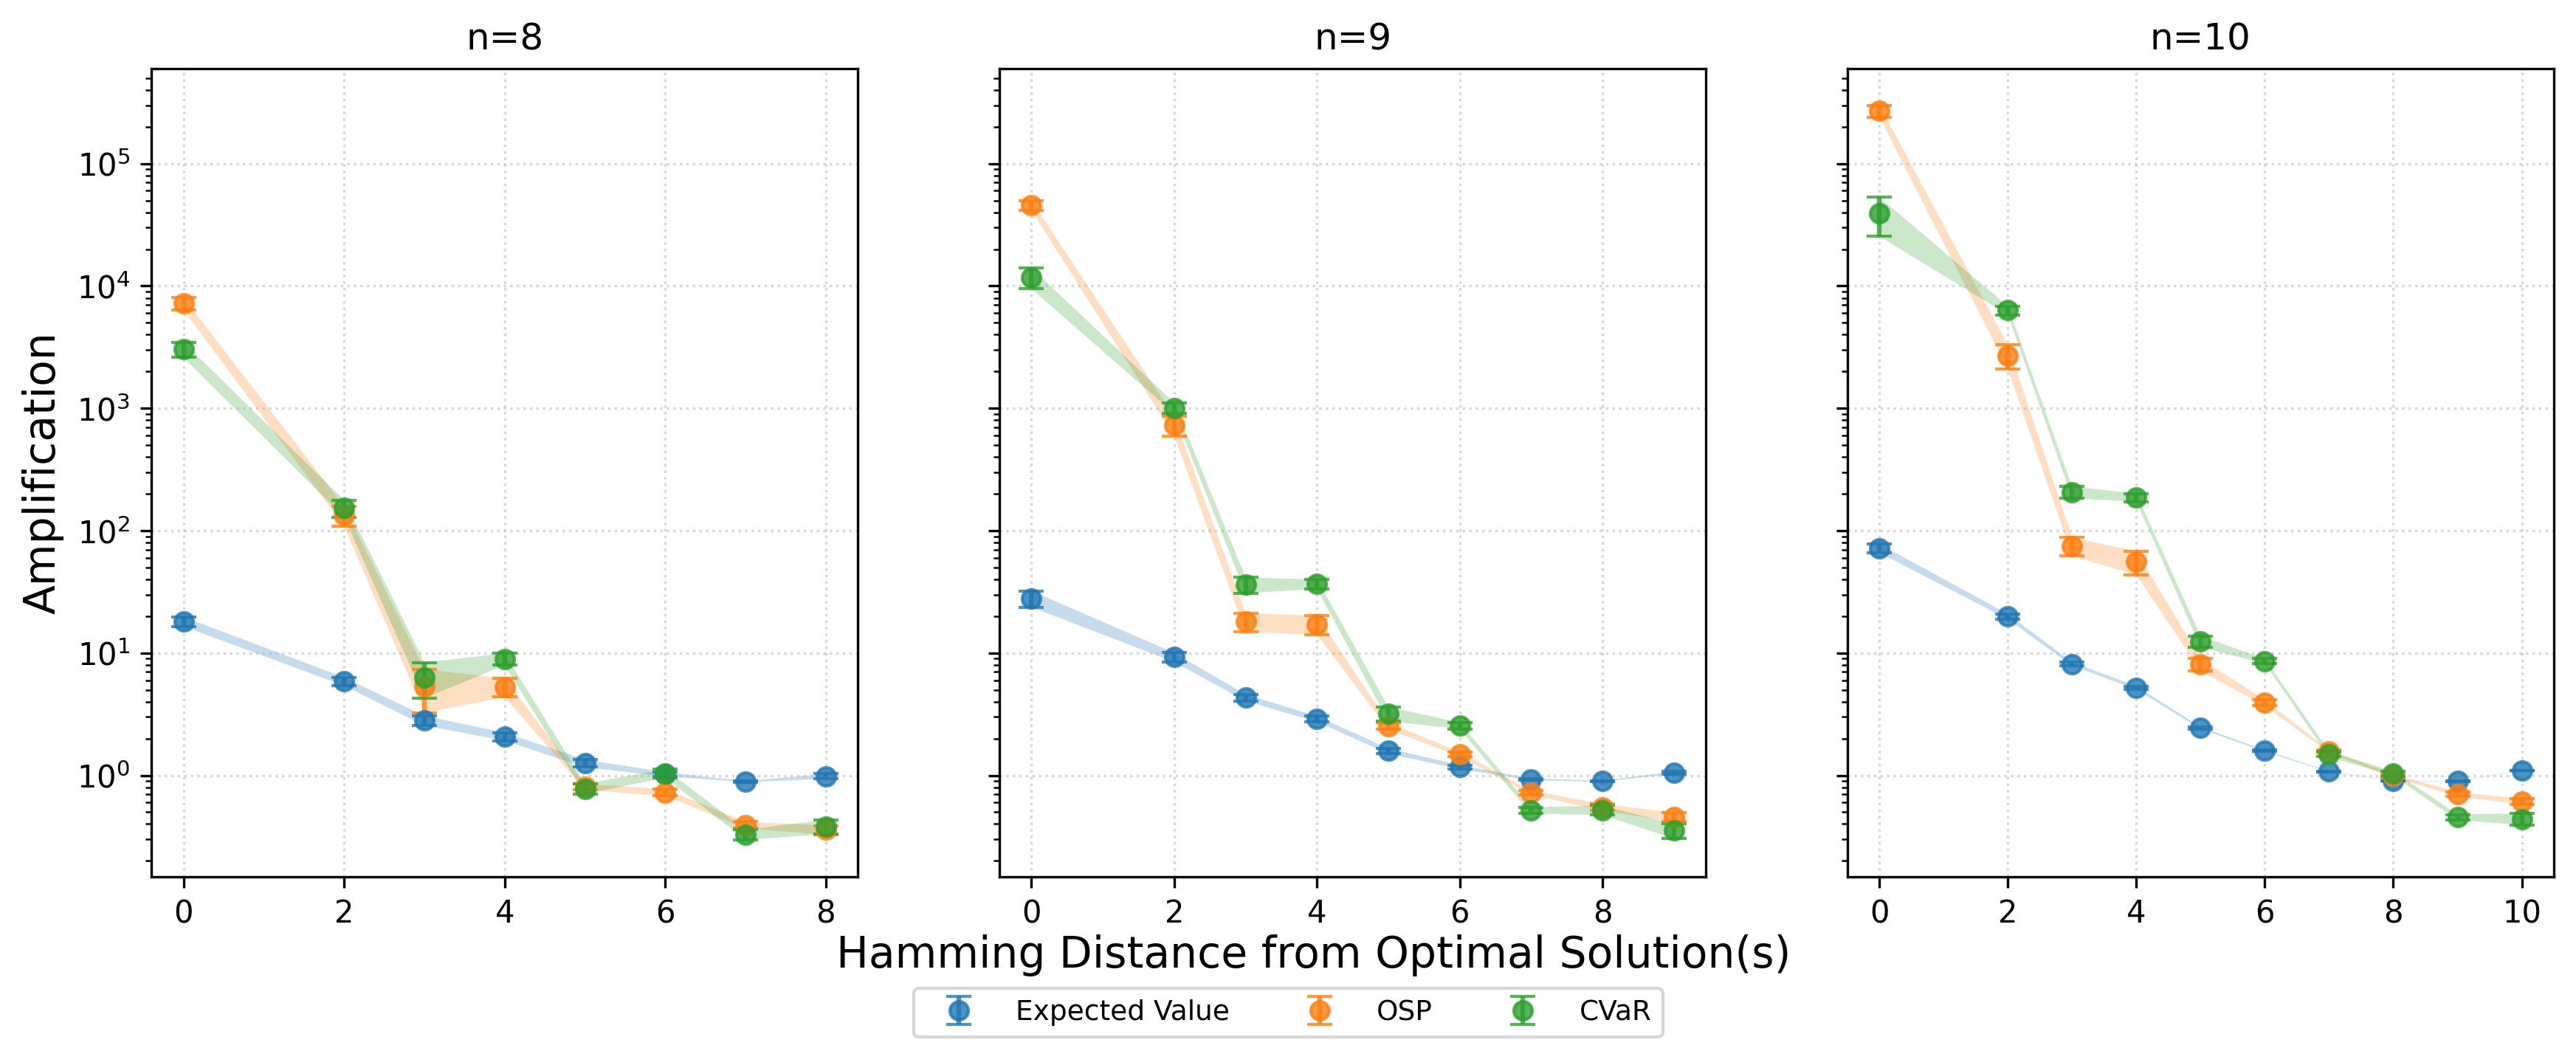
\includegraphics[width=\textwidth]{amplification_vs_hamming_multiple.png}
    \caption{Mean amplification applied to each solution grouped by their Hamming distance from the optimal solution.}
    \label{fig:amp vs ham}
\end{figure}

We also analysed the subshell distance between each solution and the optimal solution(s), which directly reflects the structure of the permutation mixer and the connectivity of the mixing graph.

Figure \ref{fig:sub improvement} shows the difference in mean subshell distance after amplification.
\begin{figure}[htbp]
    \centering
    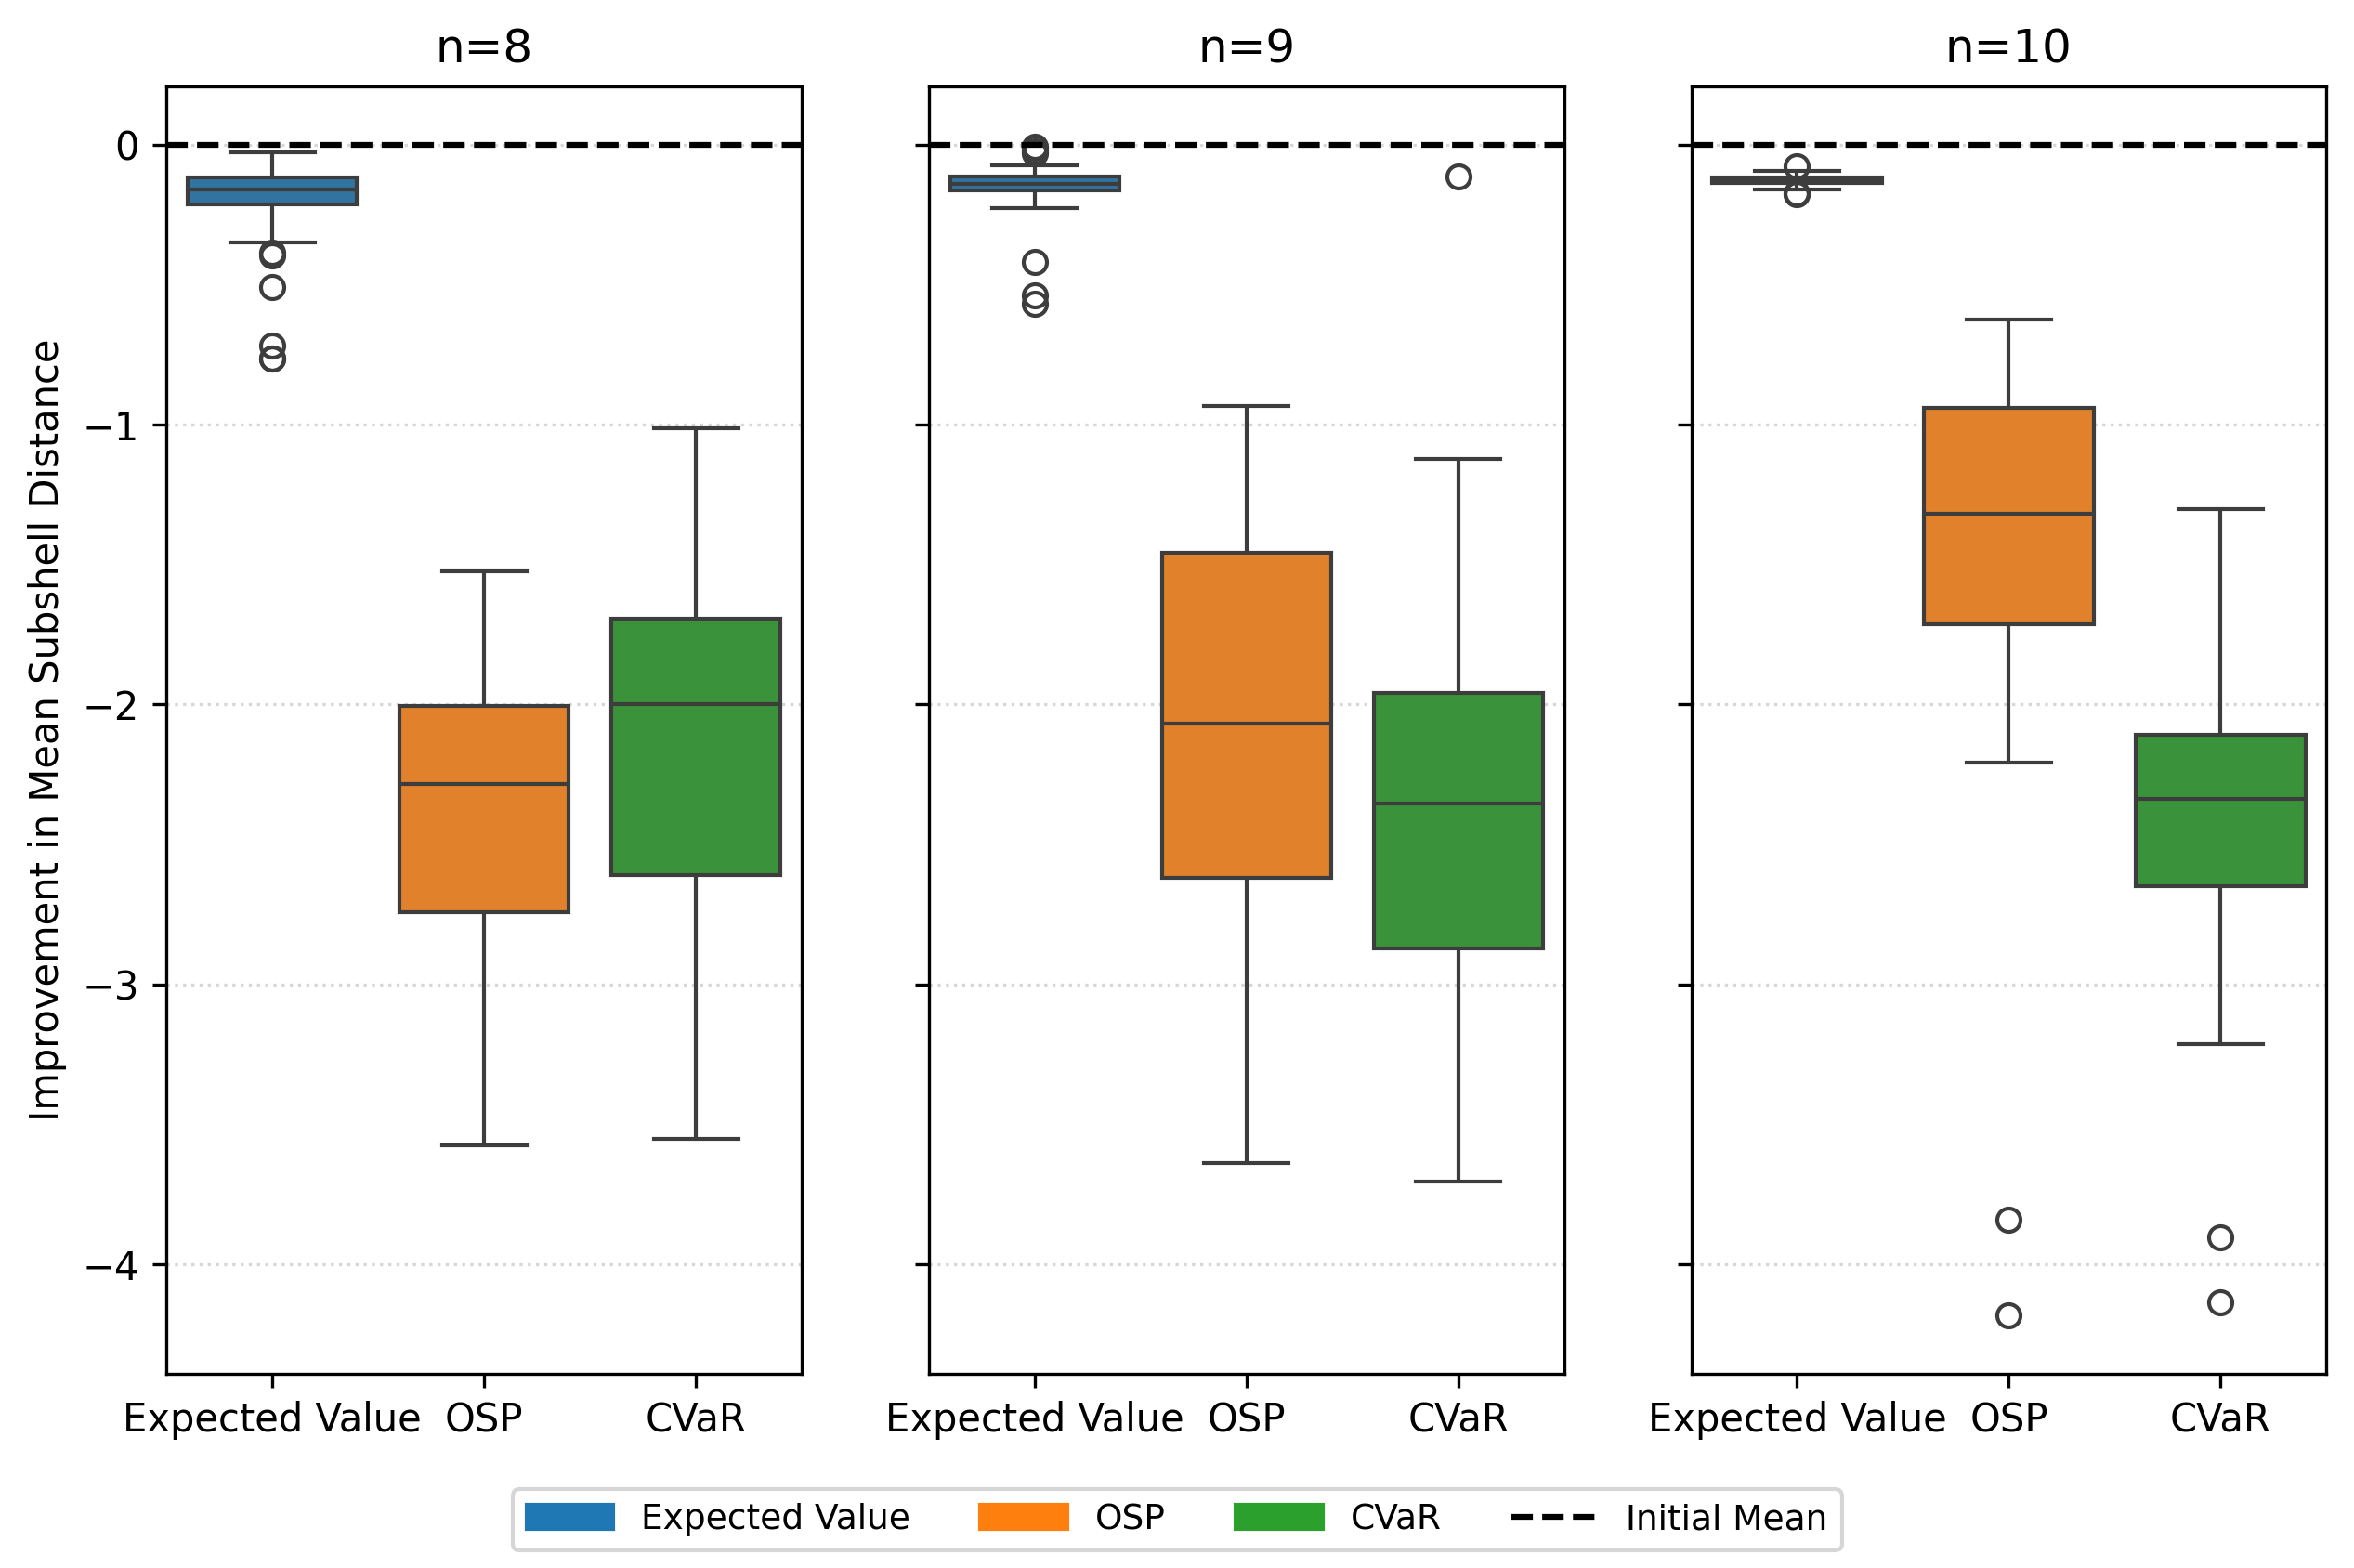
\includegraphics[width=\textwidth]{subshell_improvement_boxplot_multiple.png}
    \caption{Improvement in subshell distance boxplot.}
    \label{fig:sub improvement}
\end{figure}

Figure \ref{fig:amp vs sub} shows how much amplification was applied to each solution based on their subshell distance. These plots are monotonically decreasing. 
\begin{figure}[htbp]
    \centering
    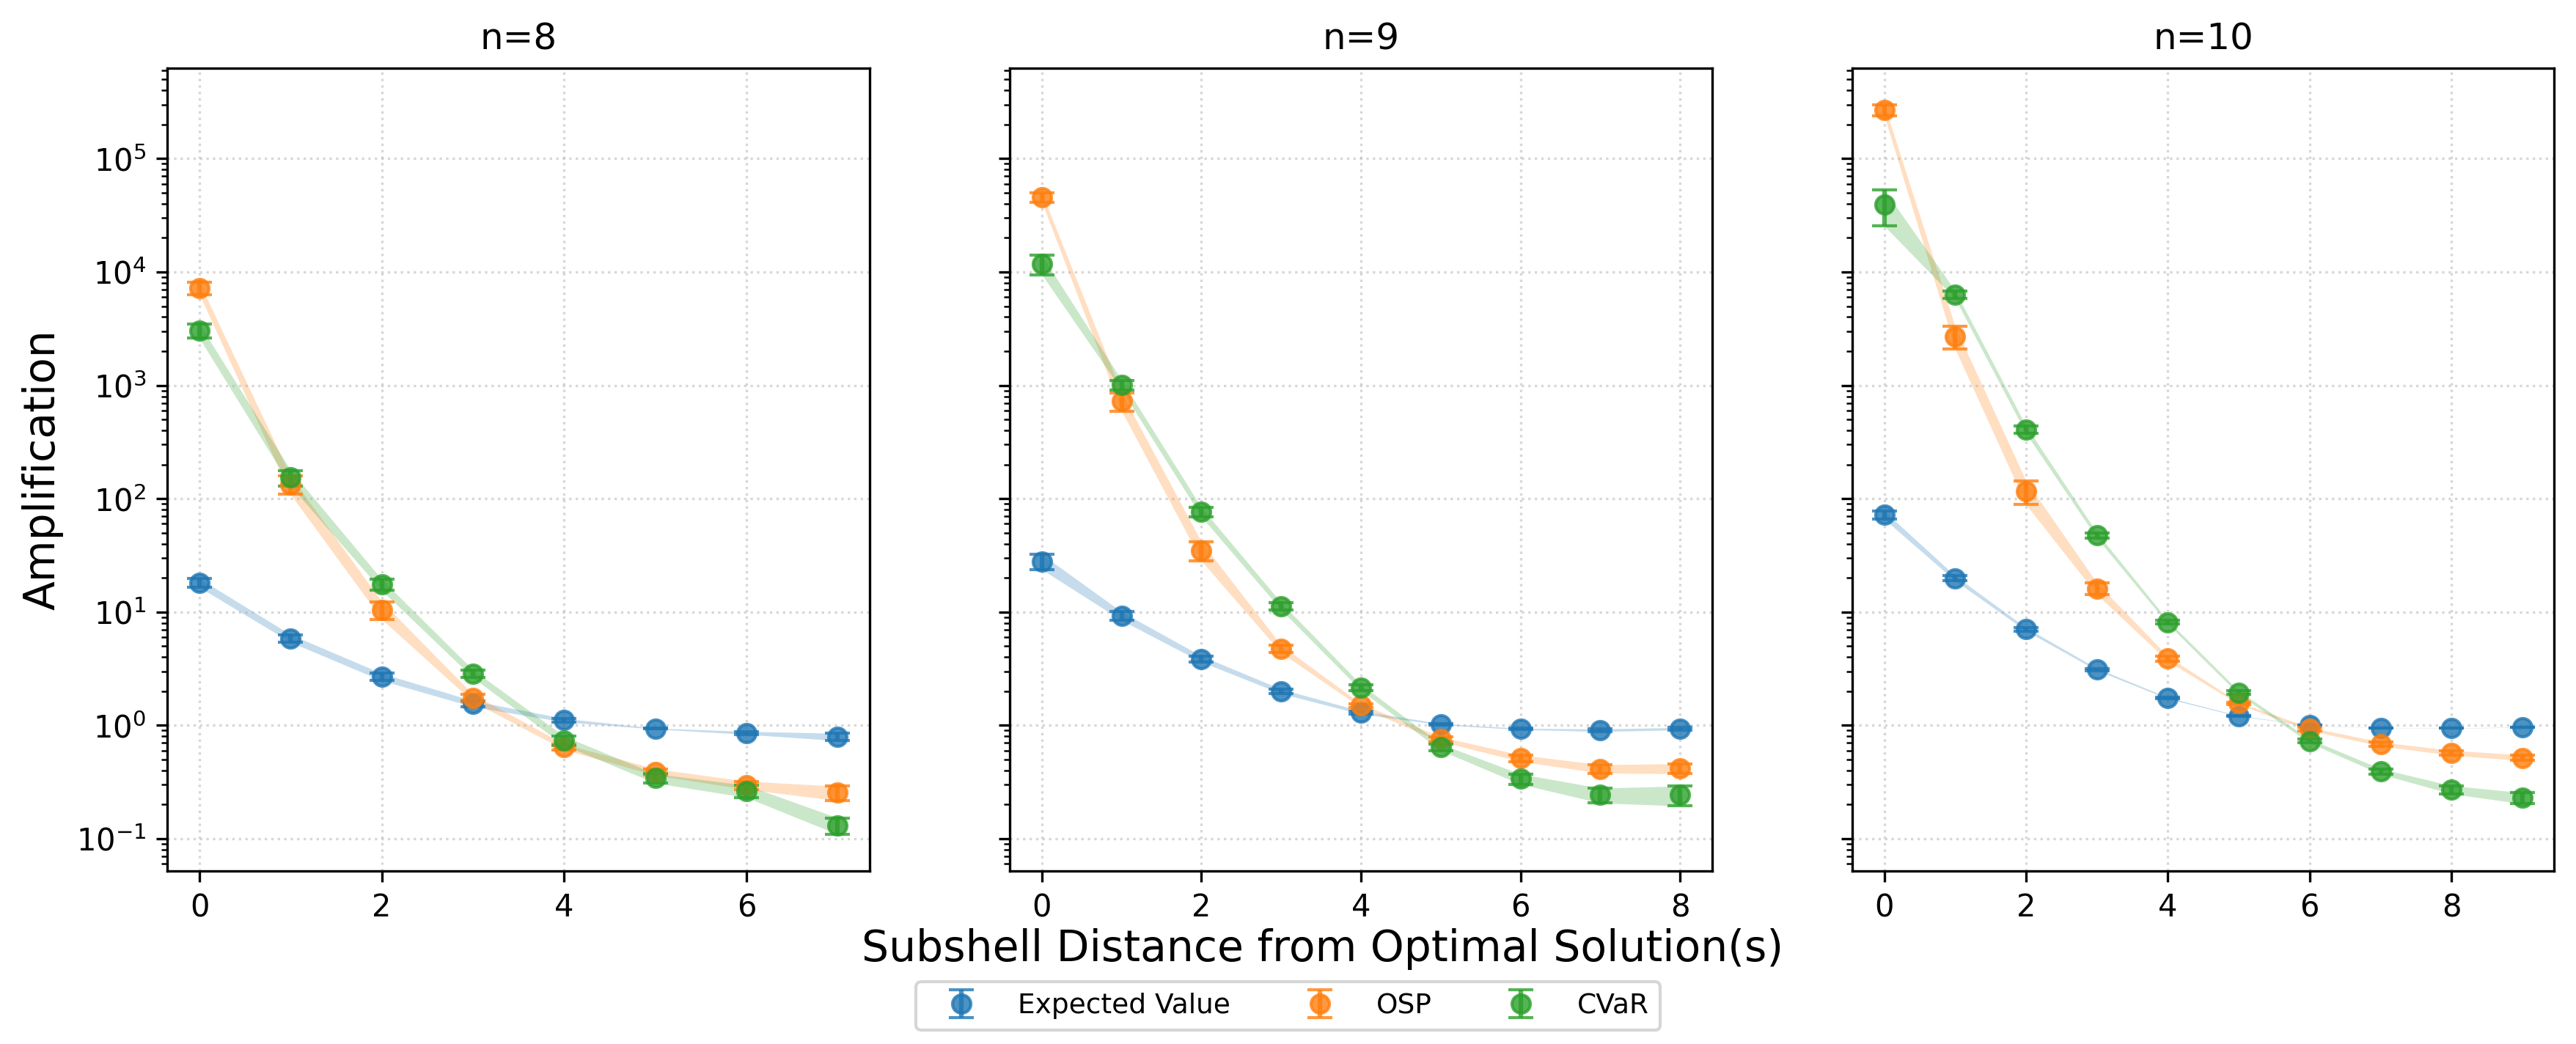
\includegraphics[width=\textwidth]{amplification_vs_subshell_multiple.png}
    \caption{Mean amplification applied to each solution grouped by their subshell distance from the optimal solution.}
    \label{fig:amp vs sub}
\end{figure}


\subsection{Hyperparameter Analysis}
We optimised the three NVQWOA hyperparameters $\beta, \gamma, t$ under three different objective functions applied to the final state: the expected value (EV), the probability of measuring an optimal solution (OSP), and the conditional value at risk (CVaR).\ref{tab:n=8}

Table of mean hyperparameters:

\begin{table}[htbp]
\begin{tabular}{c||l|l|l}
   $n=8$ & $\beta$ & $\gamma$& $t$     \\\hline\hline
    EV   & 0.47(5) & 0.2(2)  & 0.09(2) \\\hline
    OSP  & 0.78(2) & 1.01(2) & 0.180(2) \\\hline
    CVaR & 0.55(2) & 1.15(3) & 0.169(3) \\\hline
\end{tabular}
\caption{Optimisation results for $n=8$. Mean hyperparameters for each optimisation objective function.}
\label{tab:n=8}
\end{table}

\begin{tabular}{c||l|l|l}
   $n=9$ & $\beta$  & $\gamma$ & $t$     \\\hline\hline
    EV   & 0.56(2)  & -1.12(9) & 0.144(7) \\\hline
    OSP  & 0.81(2)  & 1.05(2)  & 0.164(2) \\\hline
    CVaR & 0.586(8) & 1.19(2)  & 0.142(2) \\\hline
\end{tabular}

\begin{tabular}{c||l|l|l}
  $n=10$ &$\beta$  & $\gamma$ & $t$     \\\hline\hline
    EV   & 0.47(6)  & -1.28(4) & 0.15(1) \\\hline
    OSP  & 0.78(2)  & 1.12(2)  & 0.151(1) \\\hline
    CVaR & 0.580(6) & 1.28(1)  & 0.124(2) \\\hline
\end{tabular}


\section{Subshell Analysis}
Figure \ref{fig:mqg} shows the mean quality gap between the optimal solutions and the subshells. For all problem instances, the mean quality gap was a monotonically increasing function with subshell distance.
\begin{figure}[htbp]
    \centering
    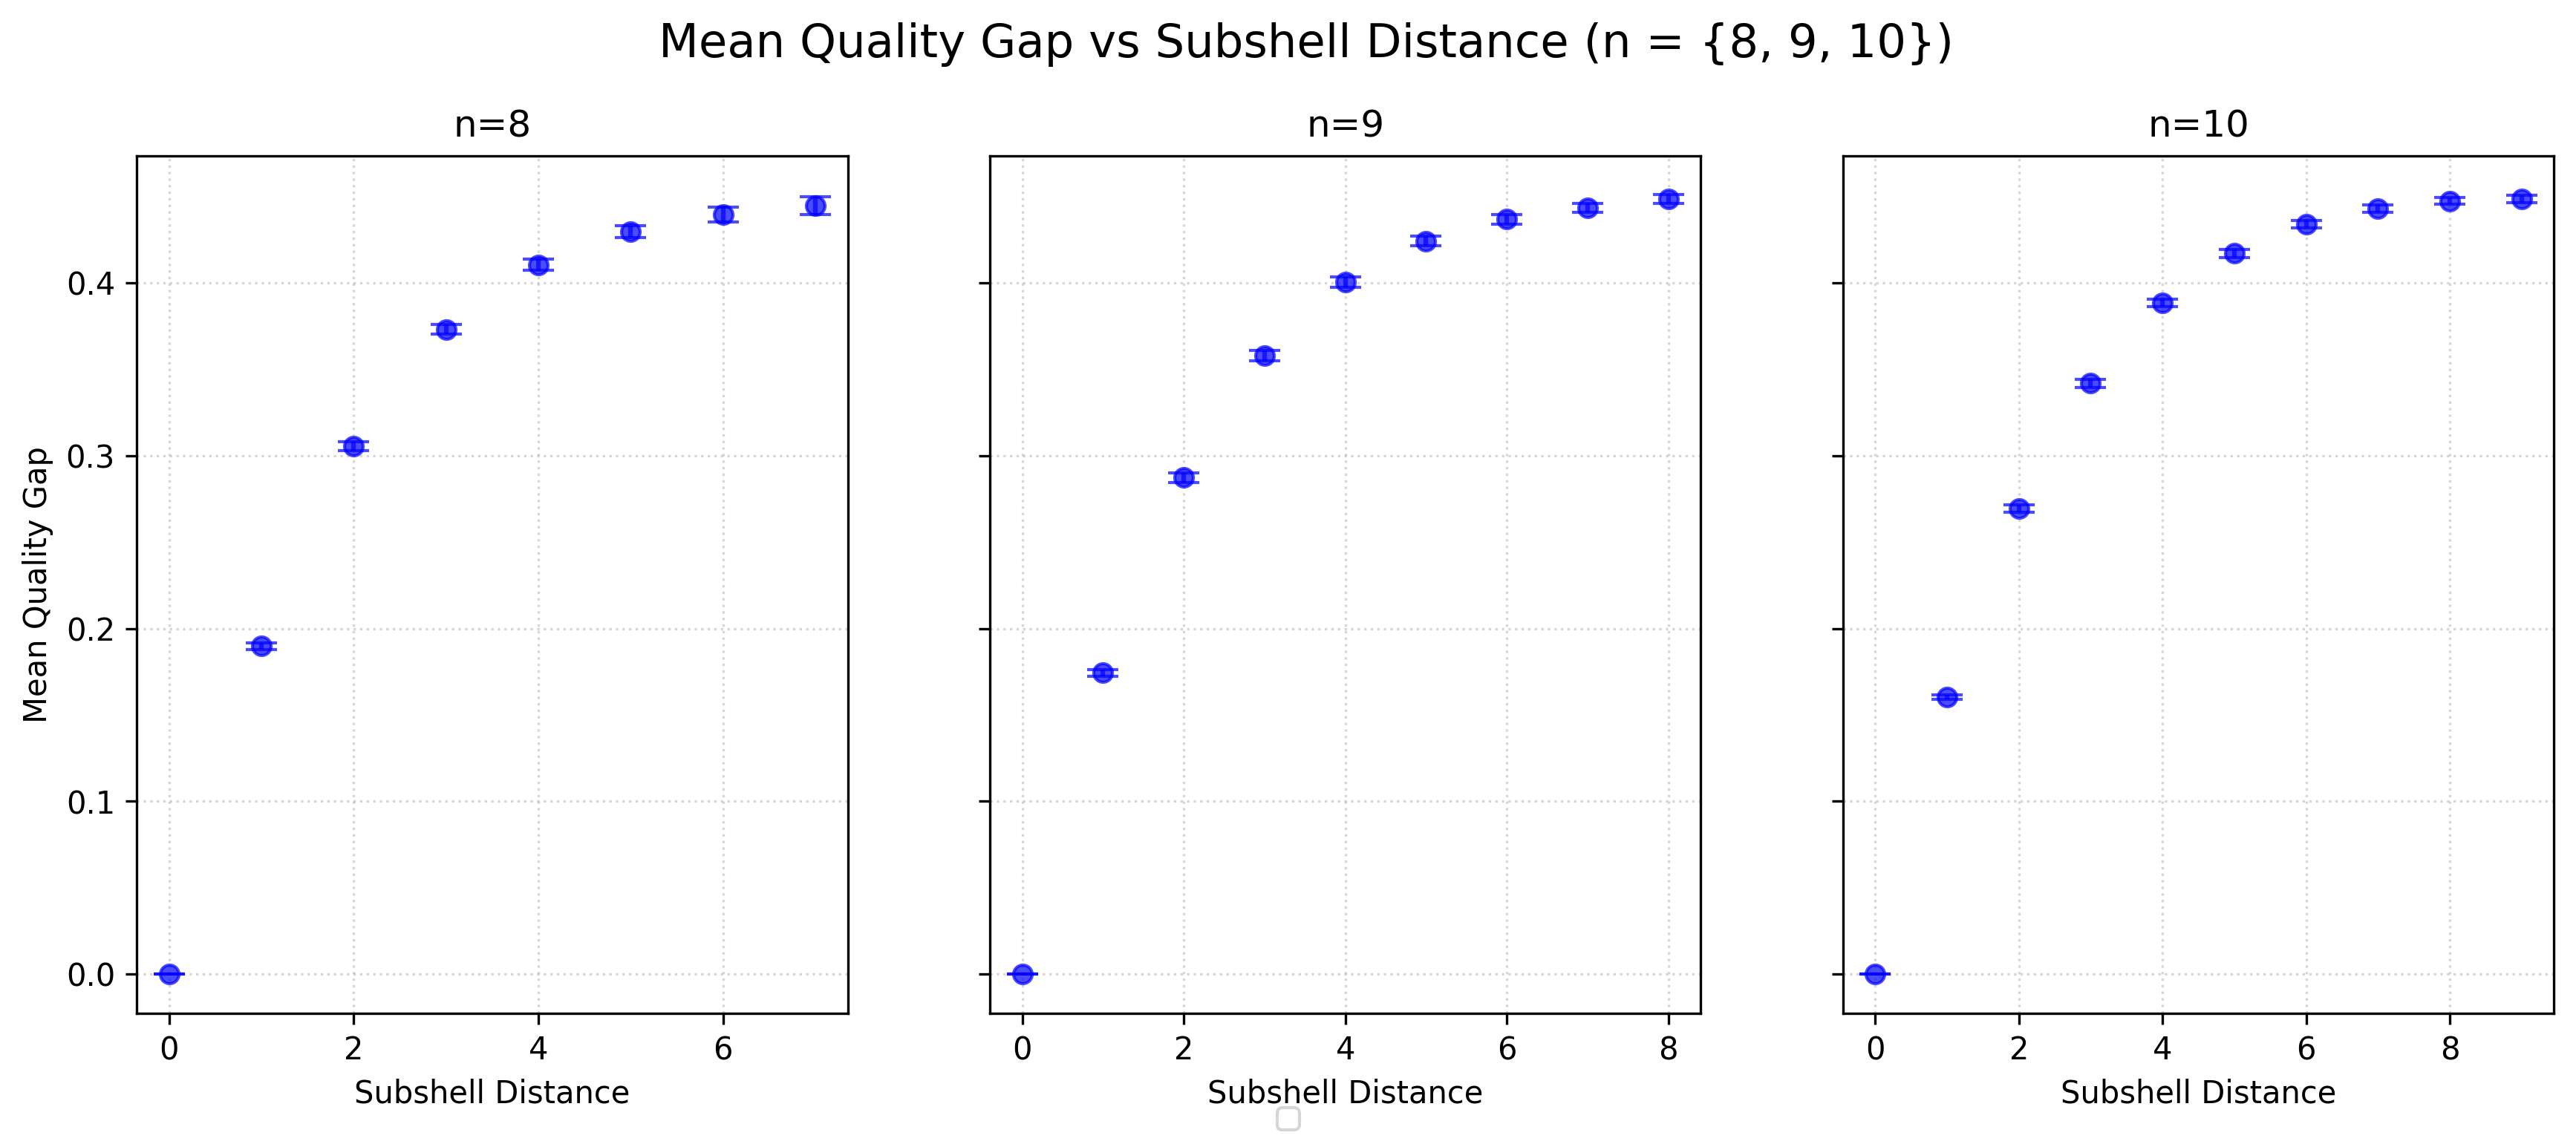
\includegraphics[width=\textwidth]{mean_quality_gap_vs_subshell_distance.png}
    \caption{Mean quality gap vs subshell distance}
    \label{fig:mqg}
\end{figure}

Figure \ref{fig:shell variance} shows the amount of variance in the objective values for each subshell.
Lower variance indicates more phase-coherence within the shell, and therefore more potential for constructive interference with the target solution under optimisation of $t$ and $\gamma$. The maximum subshell variance was X, for subshell $h$ in problem $k$. FIND THIS

The second-order variance for $n=8$ was 4.7e-06, $n=9$ was 3.2e-06, $n=10$ was 2.0e-06.
\begin{figure}[htbp]
    \centering
    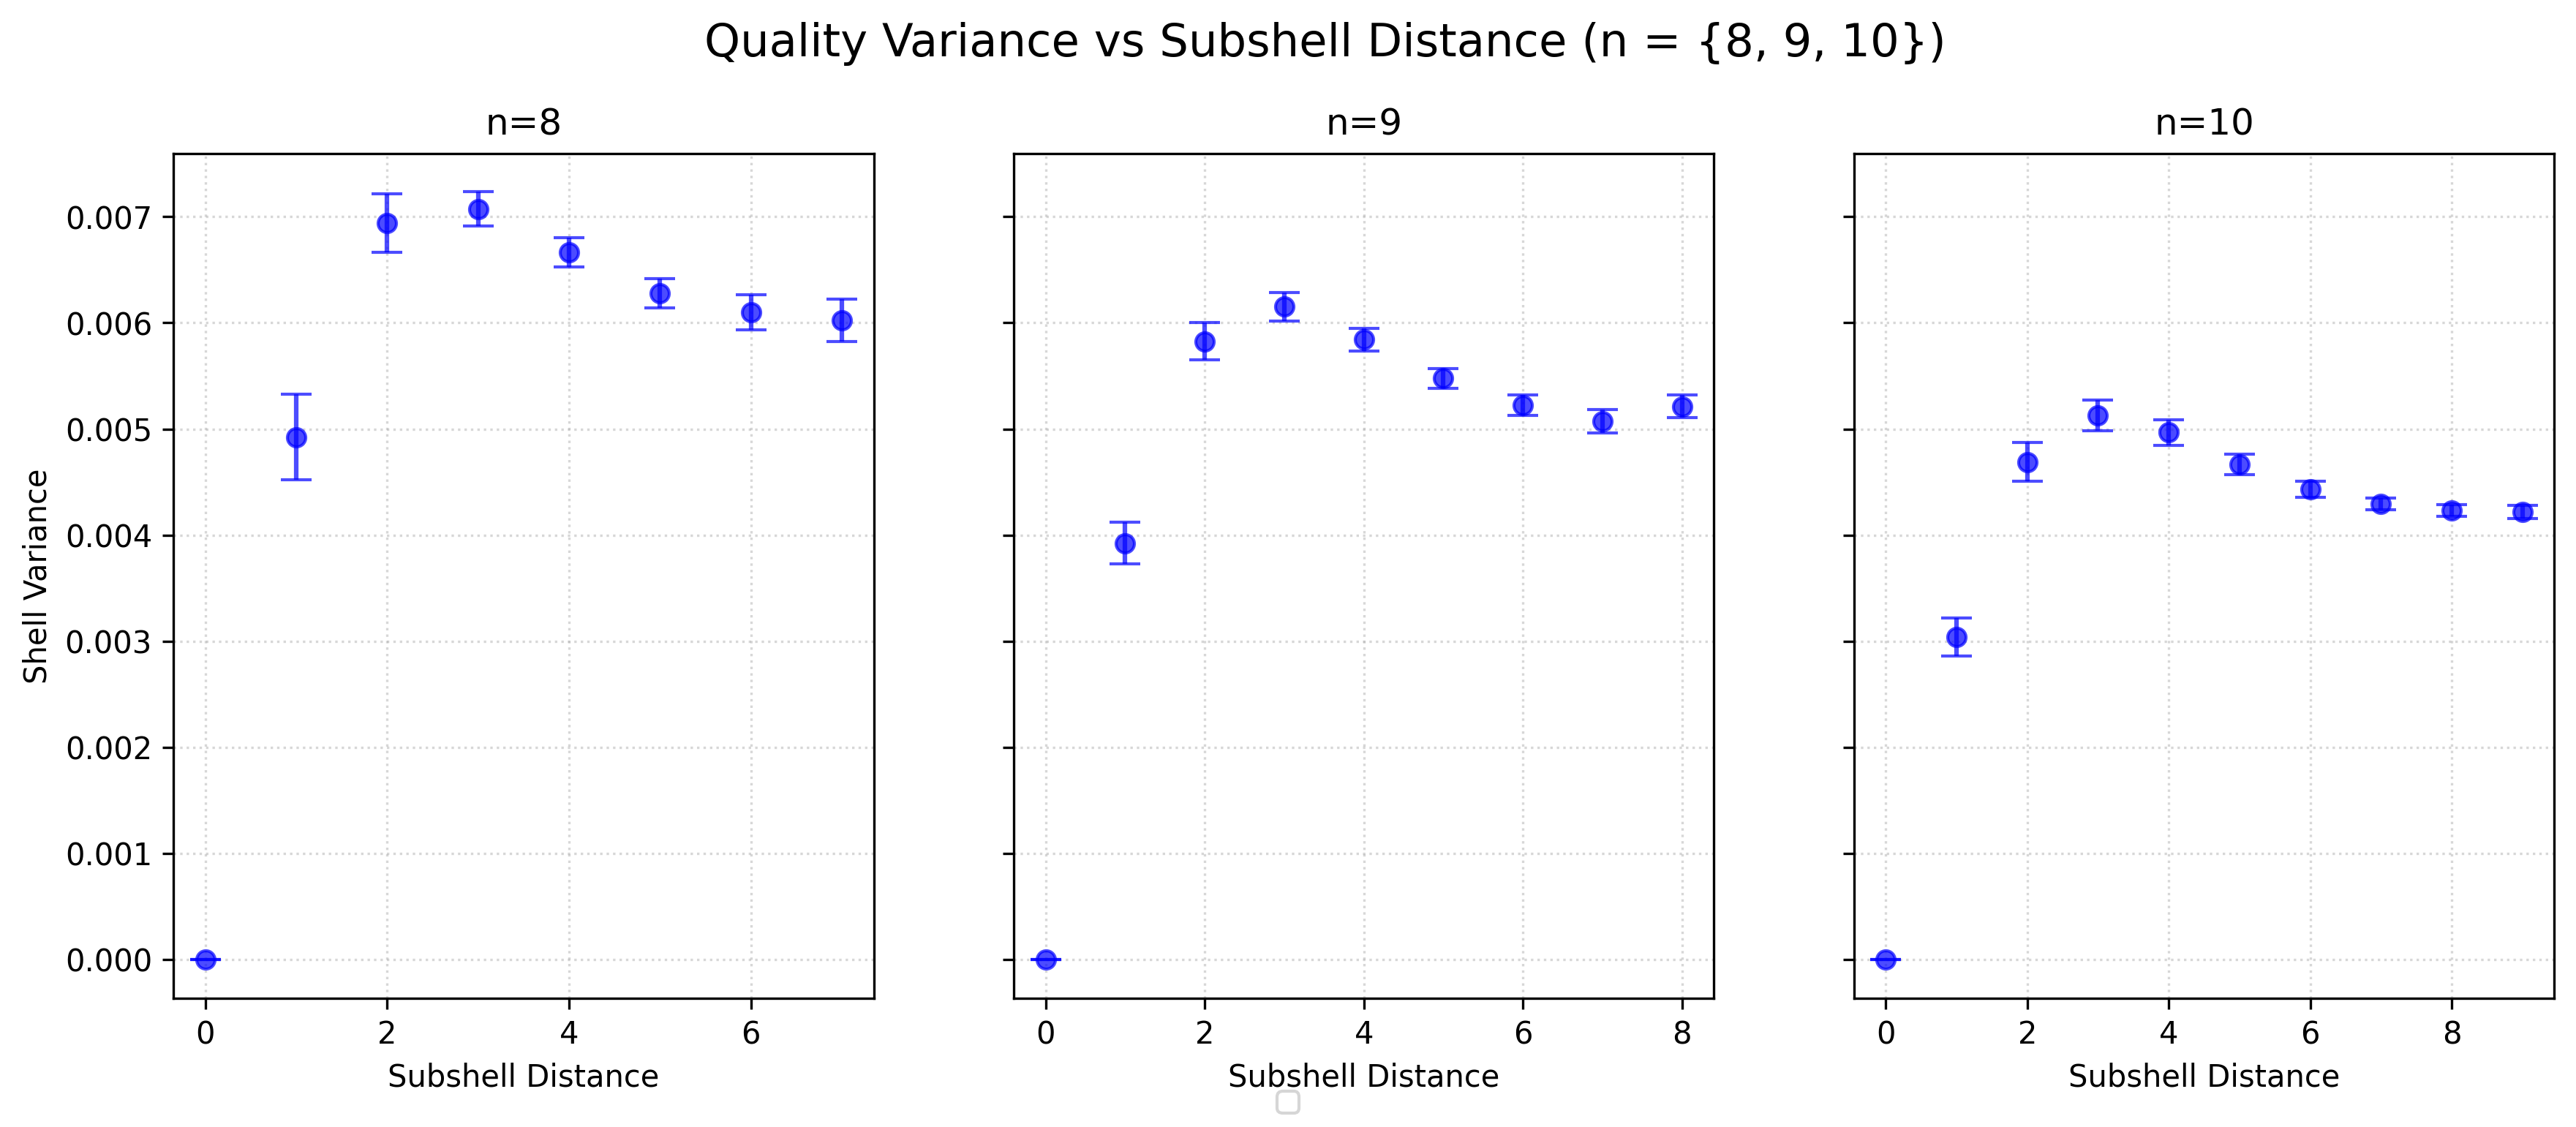
\includegraphics[width=\textwidth]{subshell_variance_multiple.png}
    \caption{Shell variance vs subshell distance}
    \label{fig:shell variance}
\end{figure}